\section{Electric Fields}

\subsection{Charge and Electric Force}

Charge is the fundamental quantity of electricity, and therefore cannot be defined. However, we can study how charges interacts. Electric charge comes in two and only two types, \textbf{positive} ($+$) and \textbf{negative} ($-$), carried by protons and electrons respectively; although the definition of which is completely arbitrary, as there doesn't exist an objective test that can be used to distinguish positive charge from negative charge, the sign of a charge can only be determined by comparison to a charge with a charge whose sign is already known. Note that the term neutral does not refer to a third type of charge, but to the presence in a region of positive and negative charges in equal amount. 

The law that governs how charged particles interact is Coulomb's Law which states: the magnitude force between two particles with charges $q_1$ and $q_2$ has the following relationship
\begin{equation}
    \| \vec{F} \| \propto \frac{q_1 q_2}{r^2},
\end{equation}
where $r$ is the distance between the centres of the particles. We measure a constant of proportionality as $k_e$, the so-called electrostatic constant. Alternatively we sometimes write the electrostatic constant in terms of vacuum permittivity $\varepsilon_0$. such that $k_e = \frac{1}{4\pi \varepsilon_0}$. 

More formally. We say the electric force $\vec{F}_{1,2}$ exerted on particle 1 due to particle 2 with charges $q_1$ and $q_2$ and position vectors $\vec{r}_1$ and $\vec{r}_2$ respectively is given by
\begin{equation}
    \label{eq:coulombs-law}
    \vec{F}_{1,2} = \frac{q_1 q_2}{4 \pi \varepsilon_0 \| r_{2,1} \|^2} \hat{r}_{2,1},
\end{equation}
where $\hat{r}_{2,1}$ is the unit separation vector pointing from particle 2 to particle 1, so we have
\begin{equation}
    \hat{r}_{2,1} = \frac{\vec{r}_{2,1}}{\| \vec{r}_{2,1}\|} \text{ and } \vec{r}_{2,1} = \vec{r}_1 - \vec{r}_2.
\end{equation}
It also follows that from Newton's third law of motion, the force on the particle with charge $q_2$ exerted by $q_1$ is given by
\begin{equation}
    \vec{F}_{2, 1} = - \vec{F}_{1, 2}.
\end{equation}
The rule of action is implied by Coulomb's Law, however, it is so fundamental that it deserves to be a law in it's own right.
\begin{theorem}{(\textbf{Rule of Action})}
\textit{The rule of action states that like charges repel and opposite charges attract.}
\end{theorem}
Electric charge is also a conserved property; the net charge (see definition \ref{def:net-charge}) of an isolated system cannot change.
\begin{definition}{(\textbf{Net Charge})}
\label{def:net-charge}
\textit{The net charge of an isolated system, $Q_{net}$, is defined as the sum of positive charges, $Q^{+}$, minus the sum of negative charges, $Q^{-}$.}
\begin{equation}
    Q_{net} = Q^{+} - Q^{-}
\end{equation}
\end{definition}

Charge is also quantized, it comes in integer multiples of individual small units called the \textbf{elementary charge}, $e$, about $1.6 \times 10^{-19}$ coulombs, which is the smallest charge which can exist (excluding quarks, see section ??). The proton has a charge of $+e$ and the electron has a charge of $-e$. The unit of electric charge is the coulomb $(C)$. Due to this property, we can the net charge of an isolated system $Q_{net}$ is,
\begin{equation}
    Q_{net} = \eta e
\end{equation}
where $\eta$ is the number of charge carriers in the system, where $\eta \in \mathbb{Z}$.

\subsection{The Electric Field}

While we need two charges to quantify the electric force, we denote the \textbf{electric field} for any single charge distribution to describe it's effect on other charges. In classical field theory, we say a charge in space produces an electric field $\vec{E}$ with spherical symmetry. We have 
\begin{equation}
    \vec{E} = \frac{q_1}{4 \pi \varepsilon_0 \| \vec{r} \|^2} \hat{r}
\end{equation}
and so we have
\begin{equation}
    \vec{E} = \frac{\vec{F}}{q_2}
\end{equation}
where $\hat{r}$ is a unit surface vector, that is $\vec{r}$ is a vector that is always perpendicular to the surface of the charge. So $\vec{r}$ is always pointing away from the charge (and towards other charges). In advanced Physics an electric field is represented as a vector field (as shown below), however, in A2 Physics we use \textit{field lines} to represent the electric field, also shown below. 
\begin{figure}[h!]
    \centering
    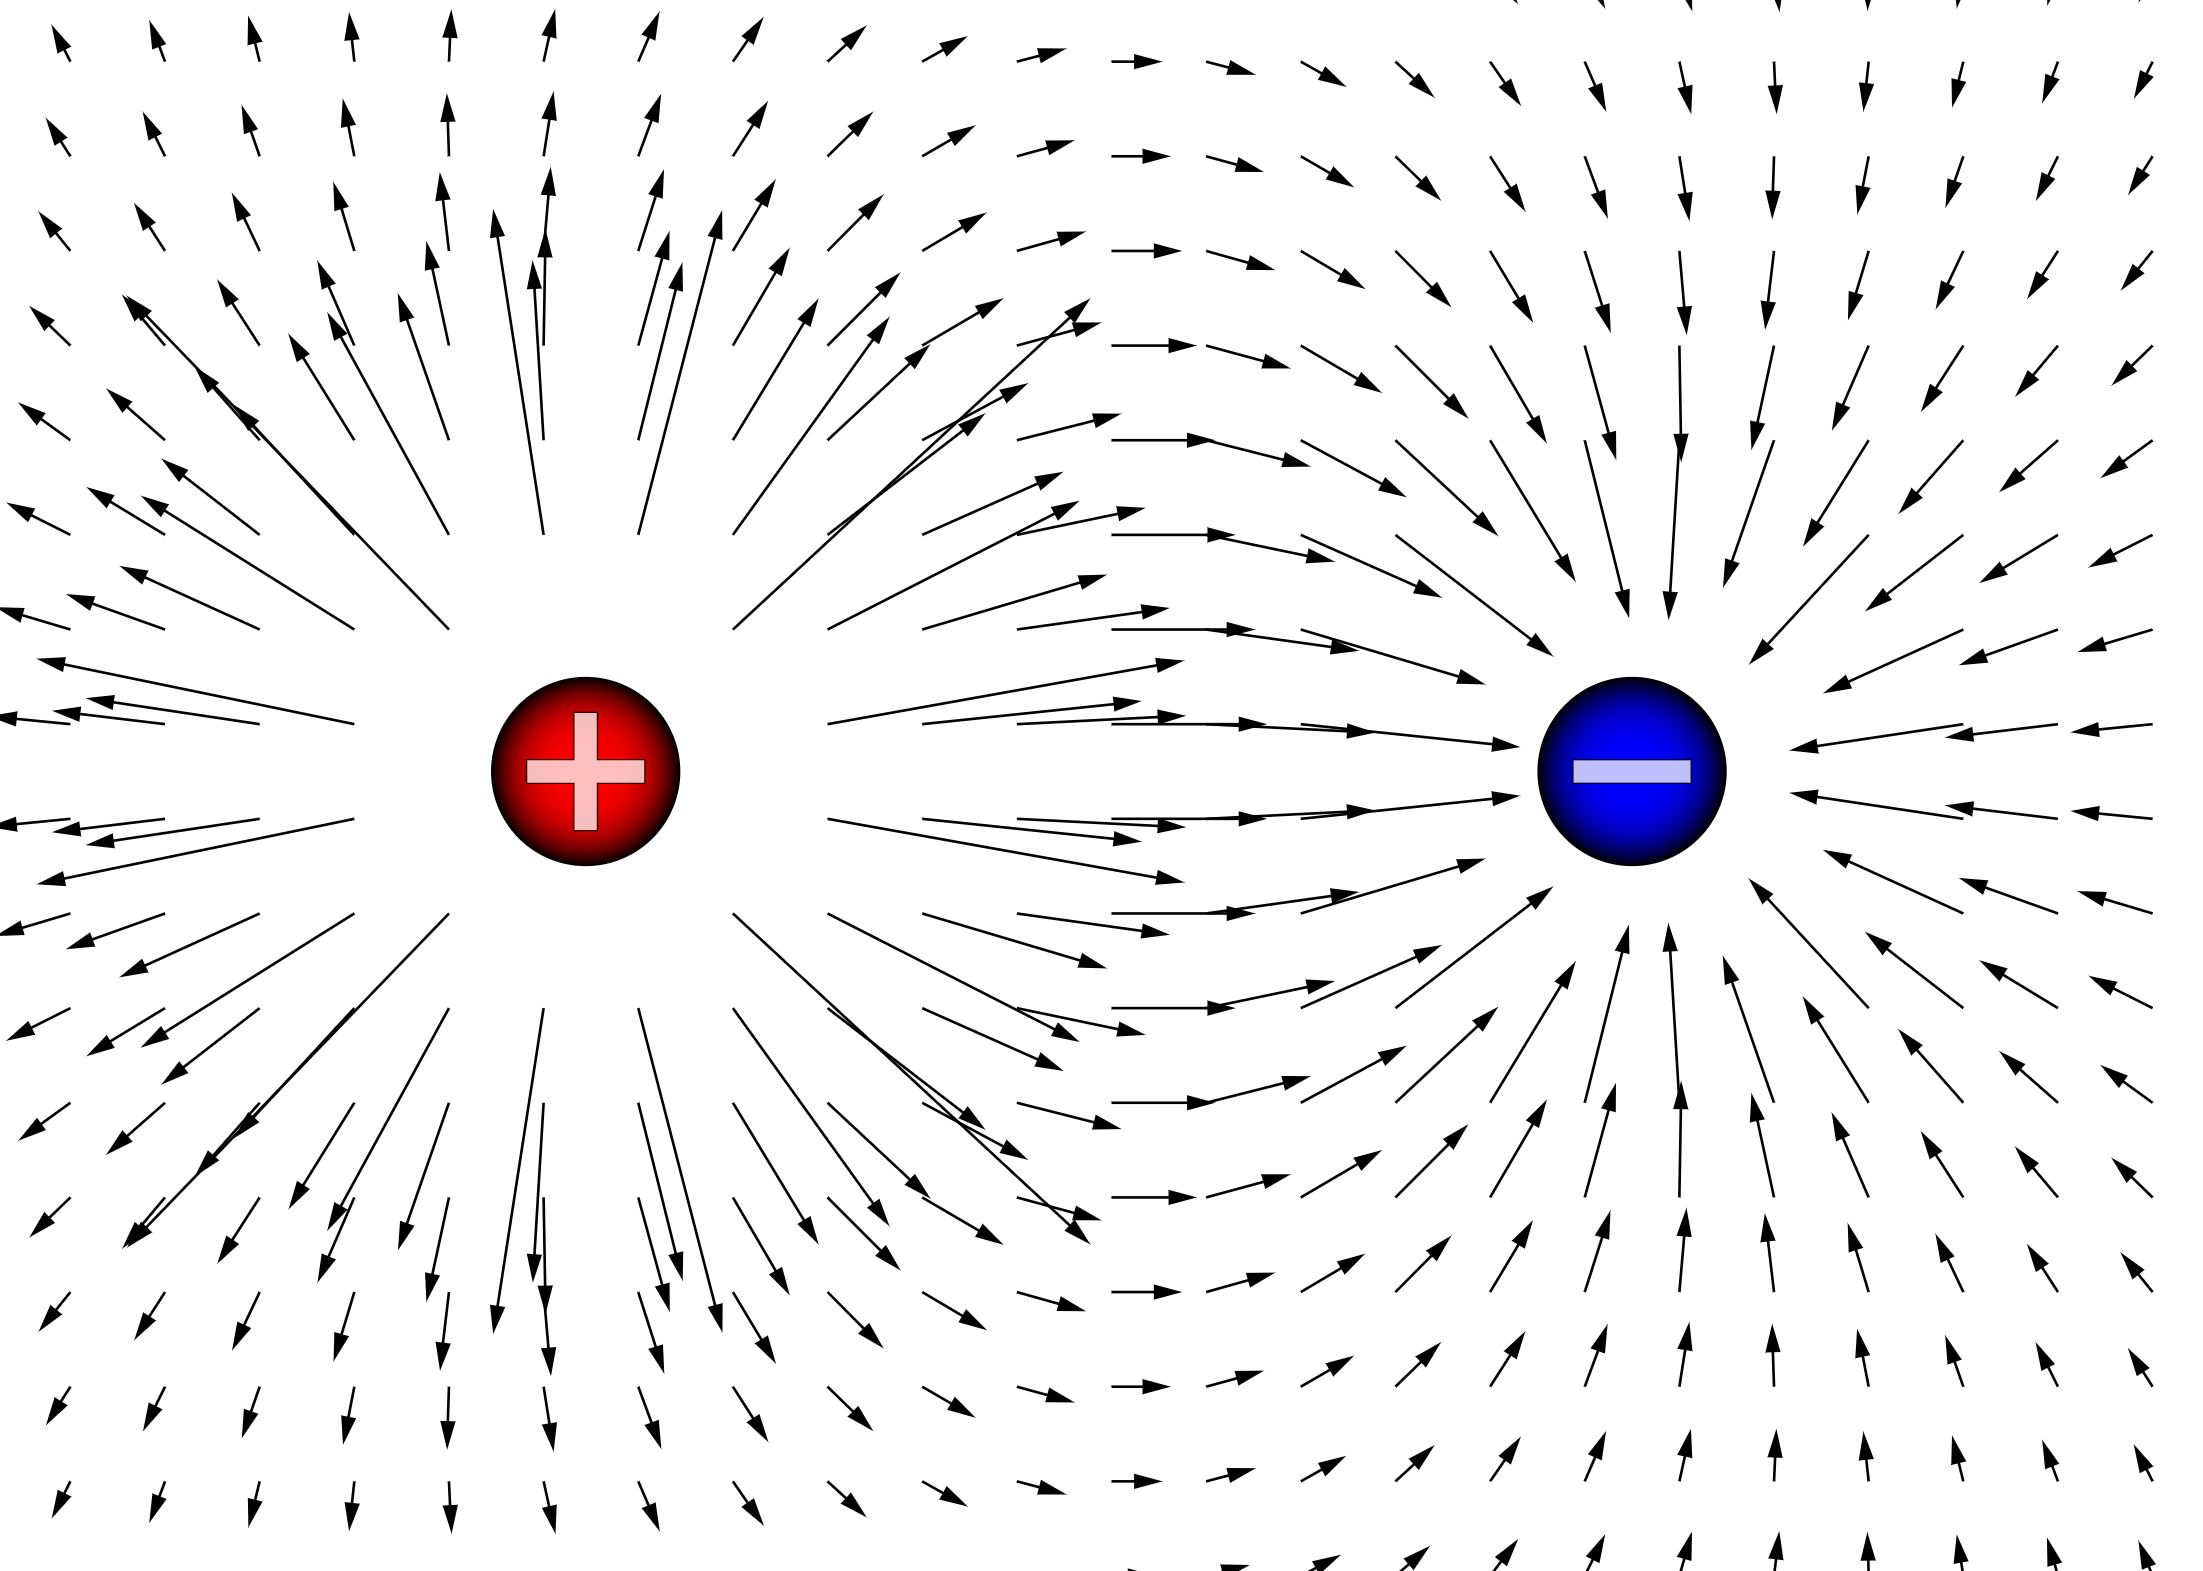
\includegraphics[scale=0.25]{notes/images/Electric-Field-Vector.JPG}
    \caption{Electric field as a vector field}
\end{figure}
\FloatBarrier

\begin{figure}[h!]
    \centering
    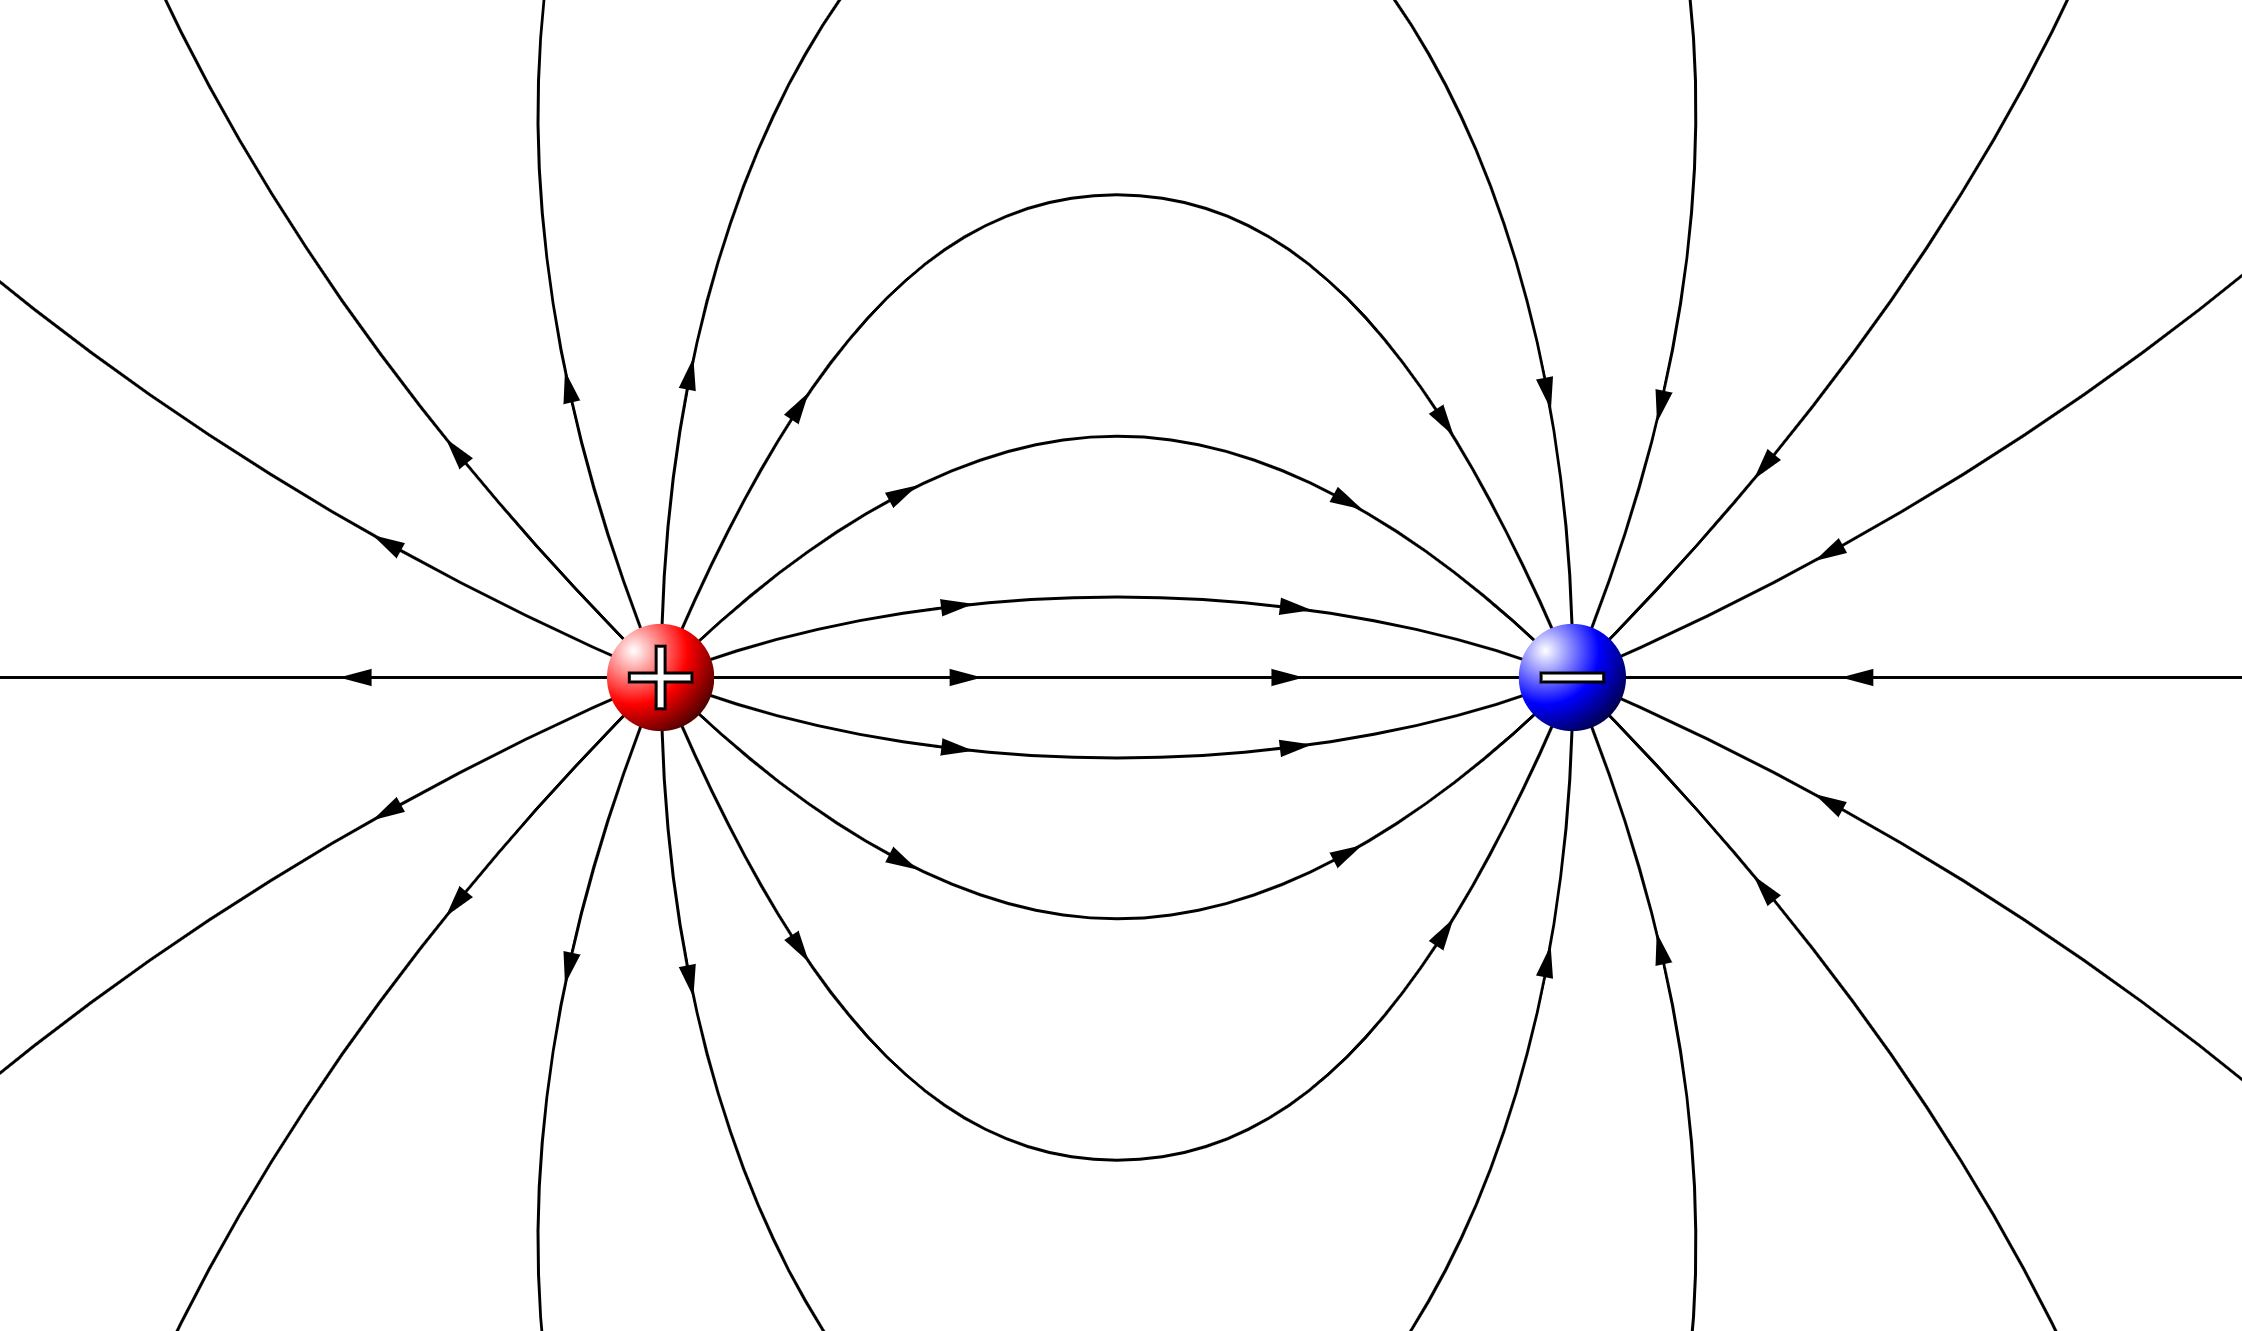
\includegraphics[scale=0.25]{notes/images/Electric-Field-Lines.JPG}
    \caption{Electric field as field lines}
\end{figure}
\FloatBarrier

The magnitude of the electric field is commonly known as the \textbf{electric field strength} and is denoted by the euclidean length of the electric field $\vec{E}$ ($\| \vec{E} \|$). 


\subsection{Potential Energy}

In general for a field, the potential $E_p$ is defined by considering the negative work done moving a charged particle from position 1 to 2, that is
\begin{equation}
    \Delta E_p = -W = - \int_C \vec{F} \cdot \mathop{\mathrm{d}\vec{s}}.
\end{equation}
Using the relations from \ref{eq:work-done-variable-force-vector} and \ref{eq:coulombs-law}, we obtain

\begin{align}
     \Delta E_p &= - \int_C k_e \frac{q_1 q_2}{\| \vec{r} \|^2} \hat{r} \cdot \mathop{\mathrm{d}\vec{s}} \\
    &= - k_e q_1 q_2 \int_C \frac{\vec{r}}{\| \vec{r} \|^3} \cdot \mathop{\mathrm{d}\vec{s}}.
\end{align}
Since $\vec{r}$ is parallel to $\mathop{\mathrm{d}\vec{s}}$, we do not need to consider a tangential vector to the curve $C$. So we have,
\begin{align}
    \Delta E_p &= - k_e q_1 q_2 \int_{r_1}^{r_2} \frac{1}{s^2} \mathop{\mathrm{d}s} \\
    &= k_e q_1 q_2 \left(\frac{1}{r_2} - \frac{1}{r_1}\right).
\end{align}

This result is generally true for both 2 and 3 dimension motion of charges. We note that it is the \textit{difference} in potential energy that is important. So we have a reference point at $r = \infty$ such that $E_p (r) = 0$. So we have
\begin{align}
    E_{p}(\infty) - E_p (r) &= - k_e q_1 q_2 \frac{1}{r} \\ 
    E_p (r) &= k_e \frac{q_1 q_2}{r}.
\end{align}

\subsection{Electric Potential}

In general for a field, the potential $V$ is defined as 
\begin{equation}
    V = \frac{E_p}{q_2},
\end{equation}
where $q_1$ is a fixed charged and $q_2$ is our so-called \textit{test charge}. So for a single point charge, the potential at a point with distance $r$ from the point charge is given by
\begin{equation}
    V = k_e \frac{q_1}{r} = \| \vec{E} \|r
\end{equation}
Recall the definition of an electric field $\vec{F} = q_2 \vec{E}$, so 
\begin{align}
    \label{eq:change-in-potential}
    \Delta V &= - \frac{1}{q_2} \int_C \vec{F} \cdot \mathop{\mathrm{d}\vec{s}} \\
    &= - \int_C \vec{E} \cdot \mathop{\mathrm{d}\vec{s}}
\end{align}
The \textbf{potential difference} is then defined (in the context of a field) as the rate of work done per unit of charge between two points around the particle of charge $q_1$. We won't evaluate this line integral in general. However, we will consider a specific case, a uniform electric field. 

Consider a path going from the $-ve$ plate to the $+ve$ plate and the potential at the point $P$, denoted $V_P$ (See figure \ref{fig:uniform-field-derivation}). 

\begin{figure}[h!]
    \centering
    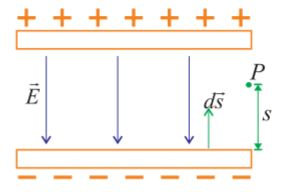
\includegraphics{notes/images/Uniform-Field-Derivation.JPG}
    \caption{A uniform field}
    \label{fig:uniform-field-derivation}
\end{figure}
\FloatBarrier

From the integral above, we'll define our initial position (at the $-ve$ plate) to have a potential of zero volts. From this we have
\begin{equation}
    \Delta V = V_p - V_{-ve} = - \int_0^s  \vec{E} \cdot \mathop{\mathrm{d}\vec{s}}. 
\end{equation}
Since $\hat{E} = -\mathop{\mathrm{d}\hat{s}}$, from this we obtain, 
\begin{align}
    V_p &= - \int_0^s (- \| \vec{E} \| ) \mathop{\mathrm{d}s} \\
    &= \| \vec{E} \| \int_0^s \mathop{\mathrm{d}s} \\
    &= \| \vec{E} \| s.    
\end{align}

Despite not evaluating the line integral above (in the general case), we can make some intuitive guesses about how it may change with respect to small changes in distance from the single point charge. We can quickly see that there exists an infinite number of positions where the potential is constant. This is due to the inverse square law of the electric field strength. The positions form a ``surface'' known as an \textbf{Equipotential surface}. Formally, an equipotential surface is a surface on which the \textit{potential is constant}. 

Having defined the concept of equipotential surfaces, we can now consider some of their properties. We note that a charge can move freely on an equipotential surface without any work done and the electric field lines must be perpendicular to the equipotential surfaces (see figure \ref{fig:equipotential}) this is because an equipotential surface has a constant potential, so the change in potential $\Delta V$ is zero. So $\vec{E} \cdot \mathop{\mathrm{d}\vec{s}} = 0$, where $\mathop{\mathrm{d}\vec{s}}$ is tangent to the equipotential surface, it follows from the definition of the dot product that $\vec{E}$ must be perpendicular to $\mathop{\mathrm{d}\vec{s}}$ and therefore perpendicular to the equipotential surface.    

\begin{figure}[h!]
    \centering
    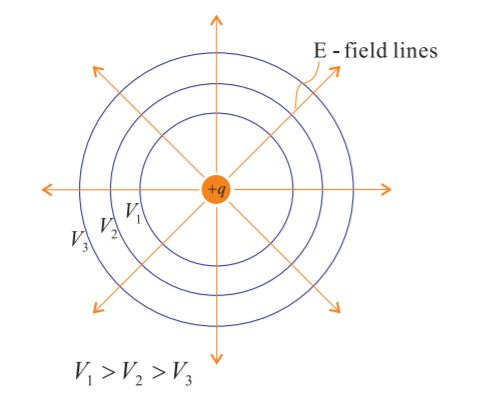
\includegraphics{notes/images/Equipotential.JPG}
    \caption{Equipotential surfaces of a point charge}
    \label{fig:equipotential}
\end{figure}
\FloatBarrier


\section{Circuits}

\subsection{Current}

\begin{definition}{(\textbf{Current})}
\label{def:current}
\textit{An electric current $I$ is defined as the rate at which charge flows through a surface (the cross section of a wire, for example).} 
\begin{equation}
    I = \frac{\mathop{\mathrm{d}Q}}{\mathop{\mathrm{d}t}}
\end{equation}
\textit{measured in \textbf{amperes} (A).}
\end{definition}

Since charge is measured in coulombs and time is measured in seconds, an ampere is the same as a coulomb per second.
\begin{equation*}
    \left[A\right] = \left[Cs^{-1}\right]
\end{equation*}
Note that this is not a definition. The ampere is a fundamental unit in the International System. Fundamental units are themselves defined by experiment. In the case of the ampere, the experiment is electromagnetic in nature. We also note, for completeness, 
\begin{equation}
    Q = \int_{t_1}^{t_2} I \mathop{\mathrm{d}t},
\end{equation}
which reduces to $Q = It$ for constant current.

\subsection{Moving Charges}

An electric current usually flows through a conductor (i.e. metals). Metals are bonded metallically, which produces \textit{delocalized} electrons which can flow freely. An electric current is created in a conductor when one end of the conductor is positive and the other is negative, it follows from the rule of action that electrons will flow to the positive end of the conductor.

\subsubsection{Conventional current}

Conventional current assumes that current flows out of the positive terminal, however, by the rule of action we know that charge carriers flow from the negative terminal to the positive terminal of the power supply.

\begin{figure}[h!]
    \centering
    \begin{circuitikz}
        \draw (0,0) to [battery](0,4) to [ammeter](4,4) -- (4,0) to [lamp](0,0);
        \draw[-latex] (4,-1) -- (0,-1);
        \node at (2, -1.5) {$\textit{electron flow}$};
        \draw[-latex] (0,-2) -- (4,-2);
        \node at (2, -2.5) {$\textit{conventional current}$};
    \end{circuitikz}
    \caption{Simple circuit with electron flow and conventional current.}
    \label{fig:conventional-current}
\end{figure}
\FloatBarrier

Although conventional current is incorrect, it makes no difference which way current is flowing as long as it is used \textit{consistently}. 

\subsection{Kirchhoff's First Law}

Kirchhoff's circuits laws are two equalities that deal with the current and potential difference (see section \ref{subsection:potential-difference}), first described by German physicist Gustav Kirchhoff. In this section, we shall discuss Kirchhoff's first law, sometimes referred to as \textbf{kirchhoff's current law}.

\begin{theorem}{(\textbf{Kirchhoff's first law})}
\textit{Kirchhoff's first law states that for any point in an electrical circuit, the sum of currents entering a given point is equal to the sum of currents leaving that point. }
\begin{equation}
    \sum I_{in} = \sum I_{out}
\end{equation}
\end{theorem}

Kirchhoff's first law can be seen as a corollary of the conservation of charge, it follows that if charge in an isolated system is constant and current is defined as the rate of which charge flows across a surface then current in an isolated system is constant, since neither charge nor time can be destroyed.

\subsection{Mean Drift Velocity}

As electrons move in a wire, they collide with positive metal ions; it follows that electrons do not have a constant velocity and not every electron has the same velocity. Hence we must consider the average, or \textit{mean}, velocity of the electrons in the wire. Although it is evident that the mean drift velocity is dependent on physical characteristics of the conductor.

\subsubsection{Classification of conductors}

A material can be classified using it's number density $n$, the number of free electrons per unit of volume, measured in $m^{-3}$. It also follows from the definition of number density that
\begin{equation*}
    n \propto \text{conductivity}.
\end{equation*}
Thus we can use number density to classify materials into conductors, semi conductors and insulators. 

\begin{table}[h!]
    \centering
    \resizebox{.6\textwidth}{!}{
    \begin{tabular}{c|c}
        \textit{Material type} & \textit{Approx. number density} ($m^{-3}$) \\
        \hline
        \textit{Conductor} & $10^{28}$ \\
        \textit{Semi-conductor} & $10^{17}$
    \end{tabular}
    }
\end{table}
\FloatBarrier

\begin{theorem}
\textit{The electric current $I$ in a conductor with cross sectional area $A$, number density $n$ and mean drift velocity of charge carriers $\overline{\vec{v}}$ is given by}
\begin{equation}
    I = Ane\|\vec{v}\|,
\end{equation}
\textit{where e is the elementary charge.}

\begin{proof}
\textit{Consider a conductor with volume $V$ $m^3$ and number density $n$ $m^{-3}$. It follows from the definition of number density and qunatization of charge that}
\begin{equation*}
    Q = neV.
\end{equation*}
\textit{Applying this to the definition of electric current, we have}
\begin{equation*}
    I = \frac{neV}{\mathop{\Delta t}}.
\end{equation*}
\textit{When there is an electric current, a certain volume of charge carriers pass through a given point each second. This volume is dependent on the cross sectional area $A$ of the conductor and the mean drift velocity of the charge carriers, so}
\begin{equation*}
    \frac{V}{\Delta t} = A\|\vec{v}\|.
\end{equation*}
\textit{Then $I = Ane\|\vec{v}\|$, thus completing the proof.}
\end{proof}
\end{theorem}

\subsection{Potential Difference and Electromotive force}
\label{subsection:potential-difference}

\begin{definition}{(\textbf{Potential Difference})}
\textit{Potential difference $V$ is defined as the rate of energy transferred $W$ per unit of charge $Q$.}
\begin{equation}
    V = \frac{\mathop{\mathrm{d}W}}{\mathop{\mathrm{d}Q}}.
\end{equation}
\textit{Alternatively (without Calculus), we have}
\begin{equation}
    V = \frac{\Delta W}{Q},
\end{equation}
\textit{measured in \textbf{volts} (V).}
\end{definition}
Since energy is measured in joules and charge is measured in coulombs, a volt is the same as a joule per coulomb.
\begin{equation*}
    [V] = [JC^{-1}]
\end{equation*}






Potential difference is sometimes described as the work done \textit{by} charge carriers, whereas, Electromotive force (e.m.f) is used to describe work done \textit{on} the charge carriers, it follows from this that Electromotive force is used when charge carriers gain energy from a source.

\begin{definition}{(\textbf{Electromotive Force})}
\textit{Electromotive force $\varepsilon$ is defined as the rate of energy $W$ transferred to electrical energy per unit of charge $Q$.}
\begin{equation}
    \varepsilon = \frac{\mathop{\mathrm{d}W}}{\mathop{\mathrm{d}Q}}
\end{equation}
\textit{measured in \textbf{volts} (V).}
\end{definition}

\subsection{The Electron Gun}

An electron gun is a device used to produce a narrow beam of electrons. In this section we will discuss the method of operation and transfer of energy that occurs in the electron gun. In later sections, we will relate the method of operation to electric fields. 

\subsubsection{Method of Operation}

\begin{figure}[h!]
    \centering
    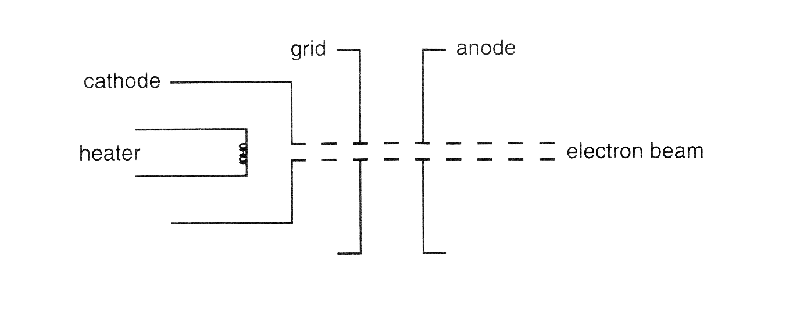
\includegraphics[scale=1.5]{notes/images/Electron-Gun.JPG}
    \caption{An Electron Gun}
\end{figure}
\FloatBarrier

\begin{enumerate}
    \item A small wire filament is heated via an electric current. The electrons in the filament gain kinetic energy ($E_k$). If the $E_k$ is large enough they escape the surface of the metal. This process is called \textit{thermionic emission} (the emission of electrons via heat). 
    \item A high potential difference (also known as the accelerating p.d) is applied to a cathode and an anode. The gun is placed in a vacuum, allowing free electrons to travel towards the anode, which is made positive with respect to the cathode, hence the electrons gain kinetic energy. 
    \item The anode has a small hole in it. So while some electrons hit the anode to return to the cell, others emerge through the hole in the anode with considerable speed.
\end{enumerate}

\subsubsection{Transfer of Energy in the Electron Gun}

The energy transferred to charges moving through a potential difference in a vacuum is transferred to the charges themselves as kinetic energy. From the definition of potential difference, the work done on a single electron travelling from the cathode to the anode is given by $eV$, where $e$ is the elementary charge and $V$ is the accelerating potential difference. 

By considering the law of conservation of energy, we can relate to the work done to the gain in kinetic energy, hence
\begin{align*}
    \text{Energy transferred to electron} &= eV \\
    &= E_k \\
    &= \frac{1}{2}m_e \| \vec{v} \|^2
\end{align*}
where $m_e$ is the mass of a single electron.

\subsubsection{Particle Accelerators}

An electron gun is a type of partial accelerator, we also have different types of particle accelerators such as \textit{linear particle accelerators} (LINACs). LINACs use a series of cylindrical electrodes (drift tubes) to accelerate subatomic particles such as electrons. The polarity off the drift tubes alternate when electrons leave the tubes thus attracting the electron to the next tube, allowing the electron to gain kinetic energy. Every time an electron moves from one tube to another it gains energy equal to $eV$. With a large number of electrodes, electrons can be accelerated to extremely high velocities. 

\subsection{Electrical Resistance}

\begin{definition}{(\textbf{Electrical Resistance})}
\textit{Electrical resistance is defined as the measure of the degree to which a conductor opposes the flow of charge carriers through that conductor,
measured in \textbf{ohms} ($\ohm$). Mathematically, the resistance R of an object is defined as the ratio of potential difference across it V to current through it I,}
\begin{equation}
    R = \frac{V}{I}
\end{equation}
\end{definition}

Since potential difference is measured in volts and current is measured in amperes, it follows that an ohm is the same as a volt per ampere.
\begin{equation*}
    [\ohm] = [VA^{-1}]
\end{equation*}

For a wide variety of materials and conditions, $V$ and $I$ are directly proportional to each other, and therefore $R$ is constant. This proportionality is called \textbf{Ohm's law}, and materials that satisfy it are called \textit{ohmic} materials.

\begin{theorem}{(\textbf{Ohm's Law})}
\textit{Ohm's law states for a metallic conductor at a constant temperature, the potential difference across the conductor is directly proportional to the current through the conductor.}

\begin{equation}
    V \propto I
\end{equation}
\end{theorem}

The \textit{current-voltage} (\textit{I-V}) graph of an ohmic conductor consists of a straight line through the origin with a positive gradient. Examples of ohmic components are wires and resistors. We should also note that ohmic conductors behave in the same way, regardless of the polarity. See Figure \ref{fig:IV-Ohmic}.

\begin{figure}[h!]
    \centering
    \begin{tikzpicture}
    \begin{axis}[
        axis lines = center,
        xlabel = $V$,
        ylabel = $I$,
        ]
        \addplot[color=red]{x};
    \end{axis}
    \end{tikzpicture}
    \caption{IV relationship of an Ohmic conductor}
    \label{fig:IV-Ohmic}
\end{figure}
\FloatBarrier

Other conductors that do not obey Ohm's law are referred to as \textit{non-ohmic}. Examples include filament lamps and diodes. See Figure \ref{fig:IV-Filament-Lamp}

\begin{figure}[h!]
    \centering
    \begin{tikzpicture}
    \begin{axis}[
        axis lines = center,
        xlabel = $V$,
        ylabel = $I$,
        ]
        \addplot[color=red]{4 * tanh(1/2 * x)};
    \end{axis}
    \end{tikzpicture}
    \caption{IV relationship of a Filament Lamp}
    \label{fig:IV-Filament-Lamp}
\end{figure}
\FloatBarrier

Notice how the filament lamp behaves in the same way, regardless of the polarity (similar to the resistor). Although in A2 a filament lamp is classified as nonohmic, if one were to consider why the p.d isn't proportional to the current we would see that as it's p.d increases, its resistance increases leading to a rise in temperature, it is this temperature that produces the non-linear increase in resistance later on. So we can conjecture that resistance is proportional to temperature.

\subsubsection{Temperature dependence}

When the temperature of a conductor increases, the positive metal ions vibrate with greater amplitude around their mean positions due to the excess thermal energy. This implies a the frequency of collisions with charge carriers and positive metal ions increases, thus an increase in the degree of which the conductor opposes the flow of charge carriers. So by definition, resistance increases.

\begin{equation}
    R \propto T
\end{equation}


\subsubsection{Resistivity}

Resistance of an object depends in large part on the material it is made of - for example, insulators have a very high resistance, while conductors have very low resistances. This material dependence is quantified by \textit{resistivity} $\rho$. The resistance of an object is dependent on three factors: the material, the length of the conductor, the cross-sectional area of the conductor. For a given conductor, the resistance $R$ is inversely proportional to the cross-section area $A$,
\begin{equation}
    R \propto \frac{1}{A}
\end{equation}
for example, a thick copper wire has a lower resistance than an otherwise-identical thin copper wire. Also, for a given material, the resistance $R$ is proportional to the length $\ell$,
\begin{equation}
    R \propto \ell
\end{equation}
for example, a long copper wire has higher resistance than an otherwise-identical short copper wire. The resistance $R$ of a conductor of uniform cross section is
\begin{equation}
    R = \rho \frac{\ell}{A}
\end{equation}
where $\ell$ is the length of the conductor, measured in metres ($m$), A is the cross sectional area of the conductor measured in square metres ($m^2$) and $\rho$ is the electrical resistivity of the material measured in ohm-metres ($\ohm m$). Based of the above equation, resistivity can be computed using 
\begin{equation}
    \rho = \frac{RA}{\ell}
\end{equation}
or resistivity can be determined by multiplying the gradient of a resistance-length (\textit{R-$\ell$}) graph by the cross-sectional area of the conductor. It follows from the above, that resistivity increases with temperature, since 
\begin{equation}
    \rho \propto R \text{ and } R \propto T.
\end{equation}

\subsection{Diodes}

A diode is a electronic component that conducts current primarily in one direction; it has a low resistance in one direction, and high (ideally infinite) resistance in the other, in other words, a diode is an electrical component that only allows a flow of current in a particular direction. It can be very useful in electronics. 

\begin{figure}[h!]
    \centering
    \begin{circuitikz}
        \draw (0,0) to [diode](3,0);
        \draw[-latex] (0,-0.5) -- (3,-0.5);
        \node at (1.5, -1) {$\textit{conventional current}$};
    \end{circuitikz}
    \caption{A Diode}
\end{figure}
\FloatBarrier

Some diodes are made of a material that  emits light when they conduct. However, unlike most light sources, these light-emitting diodes (LEDs) emit a light of a single specific wavelength, hence LEDs are extremely efficient. 

\begin{figure}[h!]
    \centering
    \begin{circuitikz}
        \draw (0,0) to [led](3,0);
        \draw[-latex] (0,-0.5) -- (3,-0.5);
        \node at (1.5, -1) {$\textit{conventional current}$};
    \end{circuitikz}
    \caption{A Light-Emitting Diode}
\end{figure}
\FloatBarrier
\noindent The \textit{current-voltage} (\textit{I-V}) graph of diode is shown below.

\begin{figure}[h!]
    \centering
    \begin{tikzpicture}
    \begin{axis}[
        axis lines = center,
        xlabel = $V$,
        ylabel = $I$,
        ]
        \addplot[color=red]{exp(x)};
    \end{axis}
    \end{tikzpicture}
    \caption{IV relationship of a diode}
\end{figure}
\FloatBarrier

\subsection{Thermistors}
\label{subsection:thermistors}

We have already seen the effect of increasing temperature increases the resistance of a conductor. Some semiconductor materials behave differently, such that their resistance drops as the temperature increases; these materials are said to have a \textit{negative temperature coefficient}. This effect can be explained using number density. As the temperature increases, the number density also increases (thermionic emission); this increase in number density increases the current flowing through the material. Given $R \propto \frac{1}{I}$, it follows that the resistance decreases. The relationship described above written in notation is shown below:
\begin{equation}
    T \propto n \propto I \propto \frac{1}{R}
\end{equation}

A thermistor is an electrical component made from a semiconductor with a negative temperature coefficient (NTC). This makes thermistors particularly useful in temperature-sensing circuits.

\begin{figure}[h!]
    \centering
    \begin{circuitikz}
        \draw (0,0) to [thR](3,0);
    \end{circuitikz}
    \caption{A Thermistor}
\end{figure}
\FloatBarrier


\begin{figure}[h!]
    \centering
    \begin{tikzpicture}
    \begin{axis}[
        axis lines = center,
        xlabel = $T$,
        ylabel = $R$,
        domain=273:573,
        samples=100,
        ]
        \addplot[color=red]{500 * exp(600 * (1/x - 1/273))};
    \end{axis}
    \end{tikzpicture}
    \caption{Resistance - Temperature relationship of a NTC thermistor}
\end{figure}
\FloatBarrier

The above relationship can be described using the $\beta$-Parameter Equation (shown below). The derivation of this relationship isn't required at A2. 
\begin{equation*}
    R = R_0 \exp\left(\beta \cdot\left(\frac{1}{T} - \frac{1}{T_0}\right)\right),
\end{equation*}
where $R_0$ is the resistance at temperature $T_0$. The semiconductor material of a thermisitor is also non-ohmic, due to the \textit{I-V} relationship shown below.

\begin{figure}[h!]
    \centering
    \begin{tikzpicture}
    \begin{axis}[
        axis lines = center,
        xlabel = $V$,
        ylabel = $I$,
        ]
        \addplot[color=red]{4 * (1/4 * x + 1/3 * (1/4 * x)^3 + 1/5 * (1/4 * x)^5 + 1/7 * (1/4 * x)^7)};
    \end{axis}
    \end{tikzpicture}
    \caption{IV relationship of a thermistor}
\end{figure}
\FloatBarrier

This relationship above can also be explained using the resistance-temperature relationship we discussed at the start of this section. As the current increases, the temperature increases, hence the resistance decreases.

\subsection{Light Dependent Resistors (LDRs)}

We saw with a thermistor how the resistance of some semiconductors varies with external factors such as temperature. A LDR uses a different type of semiconductor whose resistance varies with light intensity, in other words, it exhibits \textit{photoconductivity}. In the dark, a LDR can have an extremely high resistance, while in the light, it can have a resistance as low as a few hundred milli-ohms.

We shall explain this property, in a similar fashion to the thermistor, using number density. If the incident light on a semiconductor exceeds a certain energy requirement (similar to the work function of a metal), photons absorbed by the semiconductor give electrons enough energy become delocalised. The resulting free electrons increases the number density of the material. As explained section \ref{subsection:thermistors}, the increase in number density decreases the resistance. Giving the following relationships,
\begin{equation}
    I_v \propto n \propto I \propto \frac{1}{R},
\end{equation}
where $I_v$ denotes the incident light intensity. A LDR is an electrical component made from a semiconductor that exhibits photoconductivity. This makes LDRs particularly useful in light-sensing circuits.

\begin{figure}[h!]
    \centering
    \begin{circuitikz}
        \draw (0,0) to [phR](3,0);
    \end{circuitikz}
    \caption{A LDR}
\end{figure}
\FloatBarrier

Experiments can be used to investigate how of an LDR varies with distance from a constant light source (see section \ref{subsection:intensity} on intensity). The results of such an experiment gives a calibration curve that relates the resistance of the LDR to the light intensity. In essence, this is similar to how we build the relationship between temperature and resistance for a thermistor. 

\subsection{Electrical Power}

\begin{definition}{(\textbf{Electrical Power})}
\textit{Electrical power is defined as the rate of energy transferred by an electrical component. It is a specific type of power (see section \ref{subsection:power}).}
\end{definition}
It follows from definition \ref{def:power}, that the electrical power $P$ of a component is given by 
\begin{equation*}
    P = \frac{\mathop{\mathrm{d}W}}{\mathop{\mathrm{d}t}} 
\end{equation*}
If we consider a constant potential difference $V$ over a given electrical component, we have 
\begin{align*}
    V &= \frac{\mathop{\mathrm{d}W}}{\mathop{\mathrm{d}Q}} \\
    \mathop{\mathrm{d}W} &= V \mathop{\mathrm{d}Q},
\end{align*}
then, from definition \ref{def:current} we get
\begin{equation*}
    P = V \frac{\mathop{\mathrm{d}Q}}{\mathop{\mathrm{d}t}} = VI.
\end{equation*}
Hence we can redefine electrical power using this equation. 

\begin{definition}{(\textbf{Electrical Power})}
\textit{The electrical power $P$ of a given electrical component with potential difference $V$ volts across it and $I$ amperes through it is given by}
\begin{equation}
    P = VI
    \label{eq:power-IV}
\end{equation}
\textit{measured in \textbf{watts} (W).}
\end{definition}

We can combine the definition of resistance to give two additional equations for power. Recall that the resistance $R$ across a given electrical component with a p.d of $V$ volts and a current of $I$ amperes is given by
\begin{equation*}
    R = \frac{V}{I}.
\end{equation*}
It follows from this that $V = IR$ and $I = \frac{V}{R}$. Substituting these equations  into our definition of electrical power gives
\begin{equation}
    \label{eq:power-I2R}
    P = I^2 R \text{ and } P = \frac{V^2}{R}.
\end{equation}

\subsection{Kirchhoff's Second Law}

\begin{theorem}{(\textbf{Kirchhoff's second law})}
\textit{Kirchhoff's second law, sometimes referred to as kirchhoff's voltage law, states the sum of potential differences is equal to the sum of e.m.fs around any closed loop. That is}
\begin{equation}
    \sum \varepsilon = \sum V
\end{equation}
\end{theorem}

Alternatively, (and perhaps more formally) the law states that the directed sum of the potential differences around any closed loop is zero
\begin{equation}
    \sum V_i = 0
\end{equation}

However, care must be taken to be consistent with signs, e.g. if e.m.fs are defined as positive then potential differences dissipated in components must be negative.

Kirchhoff's second law is consistent with the conservation of energy. Since emf is the rate of energy transferred to charges and potential difference is the rate of energy transferred by the charges, it follows that they are equal. 

\subsection{Combining Resistors}

Different combinations of resistors in series and parallel can be used to build complex \textbf{resistor circuits}. Simplifying these circuits will allow us to analyze them effortlessly. In this section we will discuss the methods for simplifying resistor circuits in series and parallel.

\begin{theorem}{(\textbf{Resistors in series})}
\textit{$n$ resistors connected in a series arrangement with resistances $R_1, R_2, \ldots, R_n$ are isomorphic to a single resistor with a resistance of $R_s$ ohms, such that}
\begin{equation}
    R_s = \sum_{k=1}^n R_k.
\end{equation}
\begin{proof}
\textit{Consider the following circuit.}
\begin{figure}[h!]
    \centering
    \begin{circuitikz}
        \draw (0,0) to (0,3) to [battery1, v=$\varepsilon$](7,3) to [short, i=$I$](7,0) to [R = $R_1$, v=$V_1$](5,0) to [R=$R_2$, v=$V_2$](3,0);
        \draw (2,0) to node[right, xshift=0.2cm]{$\cdots$}(2,0);
        \draw (2.2,0) to (2,0) to [R=$R_n$, v=$V_n$](0,0);
    \end{circuitikz}
\end{figure}
\FloatBarrier
\noindent \textit{Applying Kirchhoff's second law, we have}
\begin{equation*}
    \varepsilon = \sum_{k=1}^n V_k
\end{equation*}
\textit{and from Kirchhoff's first law, the current through each resistor is equal. If we now apply Ohm's law, we obtain}
\begin{align*}
    I R_s &= \sum_{k=1}^n I R_k \\
    R_s &= \sum_{k=1}^n R_k
\end{align*}
\end{proof}
\end{theorem}
\clearpage
\begin{theorem}{(\textbf{Resistors in parallel})}
\textit{n capacitors in parallel with resistances $R_1, R_2, \ldots, R_n$ are isomorphic to a single resistor with a resistance of $R_p$ ohms, where}
\begin{equation}
    \frac{1}{R_p} = \sum_{k=1}^n \frac{1}{R_k}.
\end{equation}
\begin{proof}
\textit{Consider the following circuit.}
\begin{figure}[h!]
    \centering
    \begin{circuitikz}
        \draw (0,0) to (0,6) to [battery1, v=$\varepsilon$](6,6) to [short, i=$I$](6,0) to (5,0) to (5,3) to [R = $R_1$, i=$I_1$, v=$V_1$](1,3) to (1,0) to (0,0);
        \draw (5,1) to [R = $R_2$, i=$I_2$, v=$V_2$](1,1);
        \draw (5,0) to node[below]{$\vdots$}(5,-0.5);
        \draw (5,-1.1) to (5,-1.5) to [R = $R_n$, i=$I_n$, v=$V_n$](1, -1.5) to (1, -1.1);
        \draw (1,0) to node[below]{$\vdots$}(1,-0.5);
    \end{circuitikz}
\end{figure}
\FloatBarrier
\noindent \textit{Applying Kirchhoff's first and second law, we have}
\begin{equation*}
    I = \sum_{k=1}^n I_k \textit{ and } \varepsilon = V_1 = V_2 = \ldots = V_n,
\end{equation*}
\textit{combining these with Ohm's Law yields}
\begin{align*}
    \frac{I}{\varepsilon} &= \sum_{k=1} \frac{I_k}{\varepsilon} \\
    \frac{1}{R_p} &= \sum_{k=1}^m \frac{1}{R_k}
\end{align*}
\end{proof}
\end{theorem}

\subsection{Internal Resistance}

A source of e.m.f always has some resistance to current within it, called its \textbf{internal resistance}. The internal resistance has two effects on the source of e.m.f:
\begin{itemize}
    \item the potential difference across the terminals (the \textbf{terminal p.d}) decreases as current increases.
    \item the source is less than 100\% as energy is dissipated in the internal resistance (as is potential, known as \textbf{lost volts}).`
\end{itemize}
The internal resistance of a source of e.m.f may be thought as a resistor with resistance $r$ ohms in series with the nominal e.m.f $\varepsilon$, as figure \ref{fig:internal-resistance-emf} shows. 
\begin{figure}[h!]
    \centering
    \begin{circuitikz}
        \draw (0,0) to [battery1, v=$\varepsilon$](0,2.5) to [R, l=$r$](0,4) to (0,5) to (3,5) to [R, l=$R$](3,0) to (0,0);
        \draw[dashed] (-1,0.5) rectangle (1,4.5);
    \end{circuitikz}
    \caption{Internal resistance and source of e.m.f}
    \label{fig:internal-resistance-emf}
\end{figure}
\FloatBarrier
From Kirchhoff's second law, the relationship between the e.m.f $\varepsilon$, terminal p.d $V$ and the lost volts $\Delta V$ is 
\begin{equation}
    \label{eq:internal-resistance}
    \varepsilon = V + \Delta V = I(R + r)
\end{equation}
This relationship is essentially a version of Ohm's Law that takes into account the internal resistance of the power source. Another way to represent this relationship is graphically. Rearranging equation \ref{eq:internal-resistance} gives 
\begin{equation}
    V = \varepsilon - rI.
    \label{eq:terminal-pd}
\end{equation}
If we now plot a \textit{voltage-current} graph using the linear equation above, the gradient of graph will be equal to the negative internal resistance $-r$ the ``voltage-intercept'' is equal to the e.m.f $\varepsilon$, see figure \ref{fig:IV-cell-relationship}.

\begin{figure}[h!]
    \centering
    \begin{tikzpicture}
    \begin{axis}[
        axis lines = left,
        xlabel = $I$,
        ylabel = $V$,
        domain=0:10,
        xmin=0, xmax=10, ymin=0, ymax=15,
        ]
        \addplot[color=red]{-0.5*x + 10};
    \end{axis}
    \end{tikzpicture}
    \caption{VI relationship of a cell with internal resistance of 0.5 ohms and e.m.f of 10 volts}
    \label{fig:IV-cell-relationship}
\end{figure}
\FloatBarrier

It is often desirable to transfer as much electrical power as possible from a source to the load circuit (in figure \ref{fig:internal-resistance-emf} we used a resistor to represent our load circuit). We will show that in order to do this, the resistance of the load must be equal to the internal resistance of the source. From equations \ref{eq:power-I2R} and \ref{eq:internal-resistance}, we have
\begin{equation*}
    I = \frac{\varepsilon}{R + r} \text{ and } P = \left(\frac{\varepsilon}{R + r}\right)^2 R.
\end{equation*}
For a given internal resistance $r$, there will exist a load resistance for which the power dissipated in the load will be at a maximum due to \textit{Rolle's Theorem}. To find this we will take the derivative of power with respect to load resistance, as follows
\begin{equation*}
    \frac{\mathop{\mathrm{d}P}}{\mathop{\mathrm{d}R}} = \varepsilon^2  \frac{\mathop{\mathrm{d}}}{\mathop{\mathrm{d}R}} \left[\frac{R}{(R+r)^2} \right]
\end{equation*}
Applying the quotient rule to this, we find that
\begin{equation*}
    \frac{\mathop{\mathrm{d}P}}{\mathop{\mathrm{d}R}} = \varepsilon^2  \frac{r - R}{(R+r)^3}.
\end{equation*}
The maximum value of $P$ occurs where $\frac{\mathop{\mathrm{d}P}}{\mathop{\mathrm{d}R}} = 0$, which occurs when $r - R = 0$, that is when $R = r$. Therefore the condition for matching the internal and load resistance will transfer the maximum electrical power to the load circuit. 

\subsection{Potential Dividers and Potentiometers}

\section{Capacitance}

\subsection{Capacitors}

Capacitors are short--term ``charge--stores'', like an electrical spring.

\begin{definition}{(\textbf{Capacitor})}
\textit{An electrical component used to store and release (separated) electrical charge, consisting of 2 metal plates separated by a layer of insulating material called a dielectric.}
\begin{figure}[h!]
    \centering
    \begin{circuitikz}
      \draw (0,0)
        to[C] (2,0);
    \end{circuitikz}
\end{figure}
\FloatBarrier
\end{definition}

When a capacitor is connected to a cell of emf $\varepsilon$ (See figure \ref{fig:capacitor}), electrons flow from the negative terminal to the right plate of the capacitor. By Kirchhoff's first law electrons must be taken from the left plate. Thus producing a negative charge on the right plate and a positive charge on the left plate. 
\begin{figure}[h!]
    \centering
    \begin{circuitikz}
        \draw (0,0) to (0,4) to [battery1, v=$\varepsilon$](4,4) -- (4,0) to [C = $C$](0,0) to node[below, pos=0.35]{$-Q$}(4,0) to node[below, pos=0.35]{$+Q$}(0,0);
    \end{circuitikz}
    \caption{Simple circuit with a capacitor.}
    \label{fig:capacitor}
\end{figure}
\FloatBarrier
When charged we say the capacitor has charge of $Q$ coulombs and a potential difference of $\varepsilon$ volts.

\subsection{Capacitance}
\begin{definition}{(\textbf{Capacitance})}
\textit{Capacitance is the charge stored per unit of potential difference, measured in \textbf{farads} ($F$). Mathematically, the capacitance $C$ of an electrostatic system is the ratio of the quantity of charge stored $Q$ to the potential difference applied $V$. }
\begin{equation}
    C = \frac{Q}{V}
\end{equation}
\end{definition}
\begin{definition}{(\textbf{Farad})}
\textit{A farad is one coulomb per volt. We note that one farad is generally considered a large capacitance.}
\begin{equation*}
    [F] = [CV^{-1}]
\end{equation*}
\end{definition}
\noindent It follows that from the definition of capacitance that
\begin{equation}
    Q = VC
\end{equation}
hence, given $C$ is constant, we have
\begin{equation}
    Q \propto V
\end{equation}
therefore the charge of a capacitor is directly proportional to the potential difference across it. Let us now consider a capacitor in terms of a uniform electric field as shown below.
\begin{figure}[h!]
    \centering
    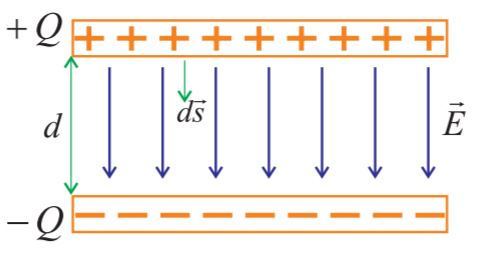
\includegraphics[scale=0.75]{notes/images/Capacitor-Electric-Field.JPG}
    \caption{Capacitor}
\end{figure}
\FloatBarrier
We will try derive capacitance in terms of the separation $d$ and the area of conducting $A$. However, we will require a new relationship that are unable to prove, as it requires knowledge of Gauss' Law which is beyond A2 Further Mathematics. 
\begin{equation}
    \label{eq:derivation-capacitance-electric-field}
    \| \vec{E} \| = \frac{Q}{\varepsilon_0 A},
\end{equation}
where $Q$ denotes charge and $A$ denotes area of conducting. Using the relationships from  \ref{eq:derivation-capacitance-electric-field} and \ref{eq:change-in-potential} and considering a path that is parallel to the electric field lines from the positive plate to the negative plate, we have
\begin{align*}
    \Delta V &= - \int_C \vec{E} \cdot \mathop{\mathrm{d}\vec{s}} \\
    &= \int_{+ve}^{-ve} \vec{E} \cdot \mathop{\mathrm{d}\vec{s}} \\ 
    &= \int_{+ve}^{-ve} \| \vec{E} \| \mathop{\mathrm{d}s} \\
    &= \frac{Q}{\varepsilon_0 A} \underbrace{\int_{+ve}^{-ve} \mathop{\mathrm{d}s}}_{\text{Length of path taken}} \\
    &= \frac{Q}{\varepsilon_0 A} d
\end{align*}
Applying the definition of capacitance to this relationship, yields a new equation for capacitance:
\begin{equation}
    C = \frac{Q}{\Delta V} = \varepsilon_0 \frac{A}{d}.
\end{equation}
When a dielectric other than a vacuum is used between the plates, the equation uses $\varepsilon$, the permittivity for the dielectric. Sometimes we use the relative permittivity $\varepsilon_r$, such that
\begin{equation}
    \varepsilon = \varepsilon_r \varepsilon_0.
\end{equation}
Therefore, the equation of capacitance may be written as
\begin{equation}
    C = \varepsilon \frac{A}{d} = \varepsilon_r \varepsilon_0 \frac{A}{d}.
\end{equation}



\subsection{Capacitors in Parallel}

\begin{theorem}{(\textbf{Capacitors in parallel})}
\textit{$n$ capacitors in parallel with potential difference $V$ across then and capacitance's $C_1, C_2, \ldots, C_n$ are isomorphic to a single capacitor with a capacitance $C_p$, where}
\begin{equation}
    C_p = \sum_{k=1}^n C_k.
\end{equation}
\begin{proof}
\textit{Consider the following circuit.}
\begin{figure}[h!]
    \centering
    \begin{circuitikz}
        \draw (0,0) to (0,6) to [battery1, v=$\varepsilon$](6,6) to [short, i=$I$](6,0) to (5,0) to (5,3) to [C = $C_1$, i=$I_1$](1,3) to (1,0) to (0,0);
        \draw (5,1) to [C = $C_2$, i=$I_2$](1,1);
        \draw (5,0) to node[below]{$\vdots$}(5,-0.5);
        \draw (5,-1.1) to (5,-1.5) to [C = $C_n$, i=$I_n$](1, -1.5) to (1, -1.1);
        \draw (1,0) to node[below]{$\vdots$}(1,-0.5);
    \end{circuitikz}
\end{figure}
\FloatBarrier
\noindent \textit{Applying Kirchhoff's first law and the definition of current to this circuit, we have}
\begin{equation*}
    I = \sum_{k=1}^n I_k \textit{ and } Q = It
\end{equation*}
\textit{combining these, it follows that}
\begin{equation*}
    Q_p = \sum_{k=1}^n Q_k
\end{equation*}
\textit{where $Q_k$ is the charge stored in the $k^{th}$ capacitor. From the definition of capacitance and Kirchhoff's second law we find that $Q_k = \varepsilon C_k$. Thus}
\begin{equation*}
    C_p = \sum_{k=1}^n C_k.
\end{equation*}
\end{proof}
\end{theorem}

\subsection{Capacitors in Series}

\begin{theorem}{(\textbf{Capacitors in Series})}
\textit{$n$ capacitors in a series arrangement with potential differences $V_1, V_2, \ldots, V_n$ across them and capacitances $C_1, C_2, \ldots, C_n$ are isomorphic to a single capacitors with a capacitance $C_s$, such that}
\begin{equation}
    \frac{1}{C_s} = \sum_{k=1}^n \frac{1}{C_k}.
\end{equation}
\begin{proof}
\textit{Consider the following circuit.}
\begin{figure}[h!]
    \centering
    \begin{circuitikz}
        \draw (0,0) to (0,3) to [battery1, v=$\varepsilon$](7,3) to [short, i=$I$](7,0) to [C = $C_1$, v=$V_1$](5,0) to [C=$C_2$, v=$V_2$](3,0);
        \draw (2,0) to node[right, xshift=0.2cm]{$\cdots$}(2,0);
        \draw (2.2,0) to (2,0) to [C=$C_n$, v=$V_n$](0,0);
    \end{circuitikz}
\end{figure}
\FloatBarrier
\noindent \textit{Applying Kirchhoff's second law, we have}
\begin{equation*}
    \varepsilon = \sum_{k=1}^n V_k
\end{equation*}
\textit{and from Kirchhoff's first law, the current $I$ entering each capacitor is equal to the current leaving each capacitor, from this it follows that each capacitor stores the same charge $Q$ coulombs. If we now apply the definition of capacitance, we find that $V_k = \frac{Q}{C_k}$, so}
\begin{align*}
    \frac{Q}{C_s} &= \sum_{k=1}^n \frac{Q}{C_k} \\
    \frac{1}{C_s} &= \sum_{k=1}^n \frac{1}{C_k}.
\end{align*}
\end{proof}
\end{theorem}

\subsection{Energy Stored in a Capacitor}

As an electron approaches the negatively charged plate of the capacitor, it experiences a repulsive electrostatic force from the electrons stored on the negative plate, so work must be done on the electron to push it onto the plate, a similar argument can be applied to pulling electrons off the positive plate. The work is provided by the cell and by the conservation of energy it follows that the energy stored in the energy stored in the capacitor is equal to the work done by the cell, which by definition is the integral of potential difference with respect to charge. 

Having rationalized this argument, we can now consider it mathematically. To charge a capacitor, we must move a small charge $\mathop{\mathrm{d}Q}$ from the $-Q$ plate  to the $+Q$ plate. This means we must do work against the potential difference, so a small amount of work $\mathop{\mathrm{d}W}$ to move a small charge $\mathop{\mathrm{d}Q}$ is given by $\mathop{\mathrm{d}W} = V \mathop{\mathrm{d}Q}$. So the total work to charge a capacitor from $0$ to $Q_1$ is given by 
\begin{equation}
    W = \int_0^{Q_1} V \mathop{\mathrm{d}Q} = \int_0^{Q_1} \frac{Q}{C} \mathop{\mathrm{d}Q} = \frac{1}{2} \frac{Q_1^2}{C} = \frac{1}{2} Q_1 V = \frac{1}{2} C V^2, 
\end{equation}
where $V$ is the potential difference across the capacitor and $C$ is the capacitance of the capacitor.

\subsection{Discharging Capacitors}
\label{subsection:discharging-capacitors}

If a capacitor is charged up by an e.m.f $\varepsilon$, then disconnected from the power supply and discharged through a resistor with resistance $R$, \textit{the charge stored will decrease exponentially}. 

We can rationalize this since as the capacitor discharges, there will be less charge stored on the plates, so the electric field strength between the plates (and thus the potential difference) will decrease. This means that the potential difference across the resistor will also decrease, and Ohm's Law predicts that then the current through the resistor will decrease too. So the rate of discharge will decrease over time. Since this rate is directly proportional to the voltage, which is in turn directly proportional to the charge stored on each plate, we have the required conditions for exponential decay. Let use analyse this a bit more mathematically, by considering the following theorem and associated proof.

\begin{theorem}{(\textbf{Discharging Capacitors})}
\textit{A discharging capacitor with capacitance $C$ and resistance $R$ in the discharge circuit can be modelled using}
\begin{equation}
    Q(t) = Q(t = 0) \exp\left(-\frac{t}{\tau}\right),
\end{equation}
\textit{where $Q(t)$ is the charge stored on each plate at time $t$ and $\tau = RC$ (the time constant).}
\begin{proof}
\textit{Let us consider a charged capacitor of $Q_0$ coulombs in the following discharge circuit}
\begin{figure}[h!]
    \centering
    \begin{circuitikz}
        \draw (0,0) to (0,2.5) to [C = $C$, v=$V$](5,2.5) to [short, i=$I$](5,0) to [R, a=$R \hspace{1mm} \ohm$](0,0);
    \end{circuitikz}
\end{figure}
\FloatBarrier
\noindent \textit{We state Ohm's Law across the resistor, $V = IR$. Now the potential difference $V$ is just $q / C$, where $q$ is the charge stored on the positive capacitor plate at some time during the discharge. Applying the definition of current to this circuit, we have}
\begin{align*}
    V &= - R \frac{\mathop{\mathrm{d}Q}}{\mathop{\mathrm{d}t}} \\ 
    \frac{1}{Q} \frac{\mathop{\mathrm{d}Q}}{\mathop{\mathrm{d}t}} &= -\frac{1}{\tau},
\end{align*}
\textit{This differential equation is solved trivially as follows}
\begin{align*}
    \int_{Q_0}^{Q_t} \frac{1}{Q} \frac{\mathop{\mathrm{d}Q}}{\mathop{\mathrm{d}t}} \mathop{\mathrm{d}t} &= - \int_0^t \frac{1}{\tau} \mathop{\mathrm{d}t} \\ 
    \int_{Q_0}^{Q_t} \frac{1}{Q} \mathop{\mathrm{d}Q} &= - \int_0^t \frac{1}{\tau} \mathop{\mathrm{d}t} \\
    \ln \left| \frac{Q_t}{Q_0} \right| &= - \frac{t}{\tau} \\
    Q_t &= Q_0 \exp \left(- \frac{t}{\tau} \right)
\end{align*}
\textit{Writing $Q_t$ explicitly as a function of time, we obtain}
\begin{equation*}
    Q(t) = Q(t = 0) \exp\left(-\frac{t}{\tau}\right).
\end{equation*}
\end{proof}
\begin{corollary}{(\textbf{Current and Voltage Equations})}
\textit{From Ohm's Law and the definition of capacitance, the decay functions for voltage and current can be derived}
\begin{equation}
    V(t) = V(t = 0) \exp\left(-\frac{t}{\tau}\right)
\end{equation}
\begin{equation}
    I(t) = I(t = 0) \exp\left(-\frac{t}{\tau}\right)
\end{equation}
\end{corollary}
\end{theorem}

Note that the we use the \textbf{time constant}. The time constant, $\tau$, is the time taken for the initial value ($Q(t = 0)$, $V(t = 0)$ or $I(t=0)$) to decrease to $\frac{1}{e} \approx 0.37$ of the initial value, hence time constant is defined as 
\begin{equation}
    \tau = RC
\end{equation}
measured in \textbf{seconds} ($s$). The time constant is the decay characteristic of these functions, similar to how half life is the decay characteristic of radioactivity. 

\subsubsection{Iterative technique for modelling exponential decay}

Instead of solving the differential equation formed in the proof above, we can apply an iterative technique to produce solutions for it. Applying the differential equation $\frac{\mathop{\mathrm{dQ}}}{\mathop{\mathrm{d}t}} = - \frac{Q}{\tau}$ to the following algorithm produces a procedure for estimating values of the decay function.

\begin{algorithm} 
    \caption{Iterative procedure for modelling exponential discharge decay function}
    \begin{algorithmic}[1]
        \Require $\tau - \text{The time constant of the discharge circuit}$
        \Require $\Delta t - \text{An incremental time period that satisfies } \Delta t \ll \tau$
        \Require $Q_0 - \text{Initial charge of the capacitor}$
        \Procedure{DecayEstimation}{$\tau, \Delta t, Q_0$}
            \If{$Q_0 \leq 0$}
                \State \textbf{return}
            \EndIf
            \State $\frac{\mathop{\mathrm{d}Q}}{\mathop{\mathrm{d}t}} \gets - \frac{Q_0}{\tau}$
            \State $\Delta Q \gets \frac{\mathop{\mathrm{d}Q}}{\mathop{\mathrm{d}t}} \Delta t$
            \State $Q_1 \gets Q_0 + \Delta Q$
            \State \textbf{output}$(Q_0, \frac{\mathop{\mathrm{d}Q}}{\mathop{\mathrm{d}t}}, \Delta Q, Q_1)$
            \State \Call{DecayEstimation}{$\tau, \Delta t, Q_1$}
        \EndProcedure 
    \end{algorithmic} 
\end{algorithm}
\FloatBarrier

\subsection{Charging Capacitors}

\begin{theorem}
\textit{A charging capacitor with capacitance $C$ and resistance $R$ in the charging circuit can be modelled using}
\begin{equation}
    Q(t) = C \varepsilon \left(1 - \exp \left( - \frac{t}{\tau} \right)\right)
\end{equation}
\textit{where $Q(t)$ is the charge stored in the capacitor at time $t$ and $\tau$ denotes the time constant.}

\begin{proof}
\textit{Imagine a DC power supply with constant e.m.f $\varepsilon$ connected in series with a capacitor $C$ and resistor $R$ (as shown below). Let $Q_0$ denote the charge of the capacitor when the potential difference across the capacitor is equal to the e.m.f (when the capacitor is fully charged), so it follows that $Q_0 = C \varepsilon$.} 
\begin{figure}[h!]
    \centering
    \begin{circuitikz}
        \draw (0,0) to [C = $C$, v=$V_C$](0,2.5) to [battery1, v=$\varepsilon$](5,2.5) to [R, l=$R \hspace{1mm} \ohm$, v=$V_R$](5,0) to [short, i=$I$](0,0);
    \end{circuitikz}
\end{figure}
\FloatBarrier
\noindent \textit{Using Kirchhoff's second law and Ohm's law, we write}
\begin{align*}
    \varepsilon - V_C &= R \frac{\mathop{\mathrm{d}Q}}{\mathop{\mathrm{d}t}} \\
    \frac{Q_0 - Q}{C} &= R\frac{\mathop{\mathrm{d}Q}}{\mathop{\mathrm{d}t}} \\
    \frac{1}{Q - Q_0} \frac{\mathop{\mathrm{d}Q}}{\mathop{\mathrm{d}t}} &= - \frac{1}{\tau}
\end{align*}
\textit{Which can be solved as shown below;}
\begin{align*}
    \int_0^{Q_t} \frac{1}{Q - Q_0} \mathop{\mathrm{d}Q} &= - \frac{1}{\tau} \int_0^t \mathop{\mathrm{d}t} \\
    \ln \left|\frac{Q_t - Q_0}{ - Q_0}\right| &= - \frac{t}{\tau} \\ 
    \frac{Q_t - Q_0}{-Q_0} &= \exp \left( - \frac{t}{\tau} \right) \\
    Q_t &= Q_0 \left( 1 - \exp \left( - \frac{t}{\tau} \right) \right)
\end{align*}
\textit{Writing $Q_t$ explicitly as a function of time, we obtain}
\begin{equation*}
    Q(t) = C \varepsilon \left( 1 - \exp \left( - \frac{t}{\tau} \right) \right)
\end{equation*}
\end{proof}
\begin{corollary}{(\textbf{Current and Voltage Equations})}
\textit{From Ohm's Law and the definition of capacitance, the exponential charging functions for voltage and current can be derived}
\begin{equation}
    V(t) = \varepsilon \left( 1 - \exp\left(-\frac{t}{\tau}\right)\right)
\end{equation}
\begin{equation}
    I(t) = \varepsilon R \left( 1 - \exp\left(-\frac{t}{\tau}\right)\right)
\end{equation}
\end{corollary}
\end{theorem}

Rationalizing these exponential charging functions can be done by considering the potential difference across and/or the current through the resistor. The current through the resistor is high initially and tends to zero as the capacitor is charged. This is because at first the capacitor is uncharged, so there is no potential difference across it and so the whole e.m.f of the supply is dissipated across the resistor. But as the capacitor gets charged, the p.d. across it opposes the e.m.f and so the p.d. across the resistor falls (since $V_0 = V_R + V_C$), as does the current (by Ohm's law). From this we can deduce that the voltage / current across the resistor can be modelled by the exponential decay equations in section \ref{subsection:discharging-capacitors}. From here the derivation is trivial. 

\section{Magnetic Force}

\subsection{Magnetic Fields}

We've seen that a particle with mass produces a gravitational field $\vec{g}$ at all points in space. In a similar manner,  a magnet is a source of a magnetic field $\vec{B}$. This can be demonstrated by moving a compass near a magnet as shown in figure \ref{fig:bar-magnet}.

\begin{figure}[h!]
    \centering
    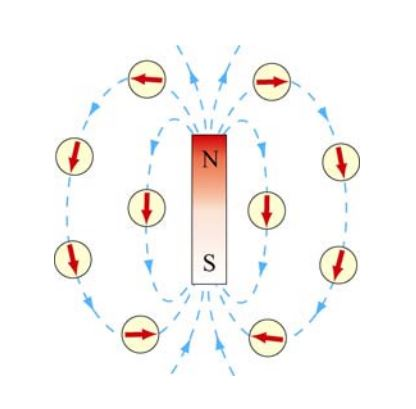
\includegraphics[scale=0.6]{notes/images/Magnetism-1.JPG}
    \caption{Magnetic field produced by a bar magnet}
    \label{fig:bar-magnet}
\end{figure}
\FloatBarrier

Notice that a magnet consists of two poles, which are designated as the north and south poles. The magnetic field lines leave from the north pole and enter the south pole. Meaning that opposite poles are attracted to each other, while the like poles will repel each other. 

\begin{figure}[h!]
    \centering
    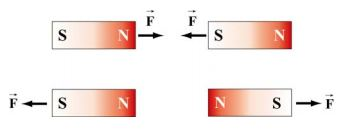
\includegraphics{notes/images/Magnetism-2.JPG}
    \caption{Magnets attracting and repelling}
\end{figure}
\FloatBarrier

Unlike a gravitational field, a magnetic field is \textbf{dipole} in nature. Meaning that magnetic ``monopoles'' do not exist in isolation. So the definition of the magnetic field $\vec{B}$ cannot exist in the following form
\begin{equation}
    \vec{B} = \frac{\vec{F}}{q_{mag}},
\end{equation}
where $q_{mag}$ is the ``magnetic charge'' of a positive magnetic test charge and $\vec{F}$ is the force acting on it. As we cannot break a magnet in half to get a north pole and a south pole. So we must look for other interactions with a magnetic force to define the magnetic field. 

It turns out that an electrically charged object (like an electron) can be accelerated by a magnetic force, and through that interaction we can define the magnetic field. To define the field at a point, consider a particle of charge $q$ and moving at a velocity $\vec{v}$. Experimentally we have the following observations:
\begin{enumerate}
    \item The magnitude of the magnetic force $\vec{F}$ exerted on the charged particle is proportional to both the magnitude of the velocity and charge.
    \item The magnitude and direction of $\vec{F}$ depends on $\vec{v}$ and $\vec{B}$.
    \item The magnitude of $\vec{F}$ is zero when $\vec{v}$ is parallel to $\vec{B}$. However, when $\vec{v}$ makes an angle $\theta$ with $\vec{B}$, the direction of $\vec{B}$ is perpendicular to the plane formed by $\vec{v}$ and $\vec{B}$ and the magnitude of $\vec{F}$ is proportional to $\sin \theta$.
    \item When the sign of the charge of the particle is switched (i.e from positive to negative), the direction of the force also reverses. 
\end{enumerate}
The above can be summarized with the following equation
\begin{equation}
    \vec{F} = q\vec{v} \times \vec{B}
\end{equation}
and the magnitude of $\vec{F}$ is given by
\begin{equation}
    \| \vec{F} \| = |q|\| \vec{v}\|\|\vec{B}\| \sin \theta
\end{equation}
The magnitude of the magnetic field $\vec{B}$, denoted $\| \vec{B} \|$, is referred to the \textbf{magnetic flux density} of the field. The $SI$ unit for magnetic flux density is the \textbf{tesla} ($T$):
\begin{equation}
    \left[T\right] = \left[\frac{N}{C \cdot ms^{-1}}\right] = \left[\frac{N}{A \cdot m}\right] = \left[kgA^{-1}s^{-1}\right]
\end{equation}

\subsection{Magnetic Fields and Work}

Let us now consider the work done on a charged particle by the magnetic force moving from position $1$ to $2$, that is
\begin{equation}
    W = \int_C \vec{F} \cdot \mathop{\mathrm{d}\vec{s}}. 
\end{equation}

Using equation ?? and re-writing $\mathop{\mathrm{d}\vec{s}}$ as $\vec{v}\mathop{\mathrm{d}t}$, we find that
\begin{equation}
    W = \int_C (q\vec{v} \times \vec{B}) \cdot \vec{v} \mathop{\mathrm{d}t}.
\end{equation}

We know that the magnetic force $\vec{F}$ is always perpendicular to velocity and the magnetic field, so from the definition of the scalar product it follows that $\vec{F} \cdot \vec{v}$ is zero. So $W = 0$ and no work is done by the magnetic field! (\textit{What a shock! How is this possible, motion with no work done!}). This implies that there is no change in energy of a charged particle being accelerated by a magnetic force, only a change in direction. 

\subsection{Magnetic Force and Circular Motion}

Recall that the magnetic force is perpendicular to the direction of motion. This implies that the trajectory of a charged particle in a uniform magnetic field is a circle in the plane perpendicular to the direction of the motion. 

Consider a charged particle with velocity $\vec{v}$ (taken to be towards the right) entering a region of uniform magnetic field point into the plane of the page. The particle will be deflected by a force that is perpendicular to the field and the initial velocity. In the example below, this will be in the upwards direction. But when recalculating the force at another point along the trajectory, we will find that the particle is continually deflect with an equal magnitude force, and the net effect is a circular orbit. Since the magnetic field does not work, the radius of the circle $r$ will be constant.

\begin{figure}[h!]
    \centering
    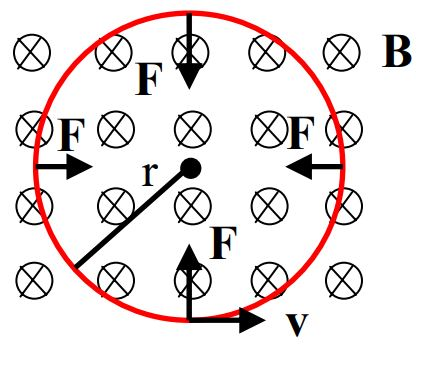
\includegraphics[scale=0.6]{notes/images/Magnetism-CM.JPG}
    \caption{Circular motion in a uniform magnetic field}
\end{figure}
\FloatBarrier

As our force acts radially, we can apply equations ?? and ?? and add a radial unit vector $\hat{r}$ to obtain
\begin{equation}
    \vec{F} = \frac{m \| \vec{v} \|^2}{r} \hat{r} = |q| \| \vec{v} \| \|\vec{B}\| \hat{r},
\end{equation}
solving for our radius $r$ of circular motion gives
\begin{equation}
    r = \frac{m \| \vec{v} \|}{|q| \| \vec{B} \|}.
\end{equation}
In other words, since momentum is defined as $\vec{p} = m \vec{v}$, we have
\begin{equation}
    r = \frac{\| \vec{p} \|}{|q| \| \vec{B} \|}.
\end{equation}
The time period for a single revolution, referred to as the \textbf{Cyclotron period}, is
\begin{equation}
    T = \frac{2\pi r}{\| \vec{v} \|} = \frac{2\pi m}{|q| \| \vec{B} \|}.
\end{equation}
    
\subsection{Lorentz Force}

In the presence of both a electric field $\vec{E}$ and a magnetic field $\vec{B}$, the resultant force, referred to as the \textbf{Lorentz force}, on the charged particle is
\begin{equation}
    \vec{F} = q(\vec{E} + \vec{v} \times \vec{B})
\end{equation}

By combining the two fields, particles can have their velocity selected. This principle was first used by J.J. Thomson to measure the charge-to-mas ratio of the electron. Figure \ref{fig:lorentz-force} illustrates Thomson's apparatus.

\begin{figure}[h!]
    \centering
    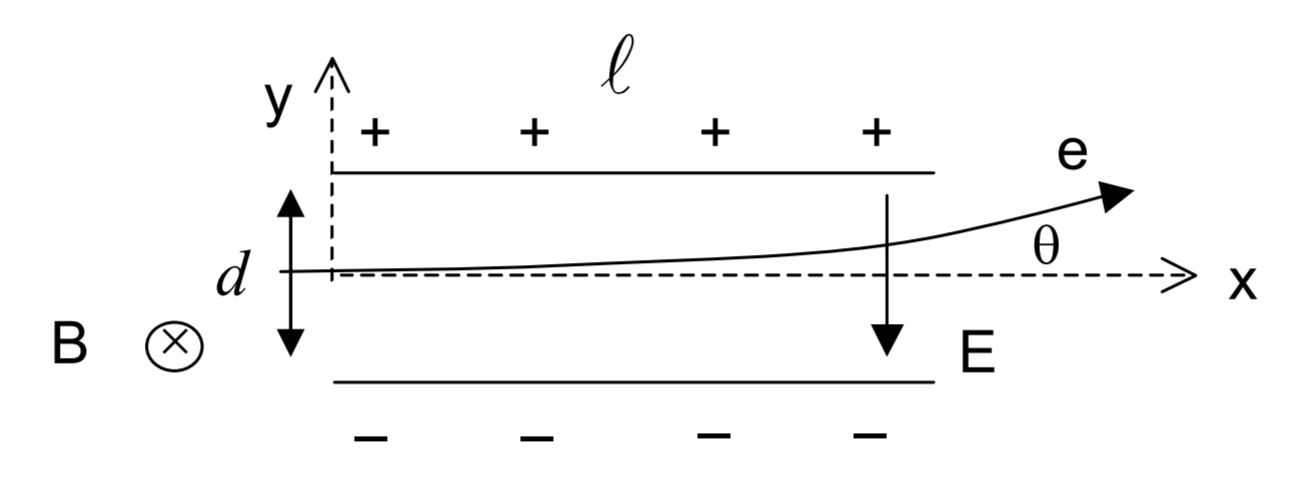
\includegraphics[scale=0.75]{notes/images/Lorentz-Force.JPG}
    \caption{Thomson's apparatus}
    \label{fig:lorentz-force}
\end{figure}
\FloatBarrier

The electrons with charge $q = -e$ and mass $m_e$ are emitted from the electron gun with velocity $\vec{v}_0$ . When the electrons pass through a region where there exists a downward uniform electric field, the electrons, being negatively charged will be deflected upwards. So only considering the electric field $\vec{E}$ we have vertical acceleration $\vec{a}_y$
\begin{equation}
    \vec{a}_y = \frac{e \| \vec{E}\|}{m_e} 
\end{equation}
    
The electric field $\vec{E}$ occupies a region of length $\ell$. We assume the electrons emitted from the electron gun only have a horizontal component for velocity. So the time to cross the region is given by
\begin{equation}
    t \approx \frac{\ell}{\| \vec{v}_0 \|}.
\end{equation}
By definition, the vertical component of velocity $\vec{v}_y$ upon exit of the region is then
\begin{equation}
    \vec{v}_y = \vec{a}_y t = \frac{e \|\vec{E}\| \ell}{m_e \| \vec{v}_0 \|}
\end{equation}
So the tangent of the exit angle is
\begin{equation}
    \tan \theta = \frac{e \| \vec{E} \| \ell}{m_e \| \vec{v}_0 \|^2}
\end{equation}
The angle $\theta$ and the length of the electric plates can be measured experimentally. The electric field strength can be determined from the potential difference applied across the plates divided by the separation, 
\begin{equation}
    \| \vec{E} \| = \frac{V}{d}
\end{equation}

We can determine the initial velocity using an energy consideration in the electron gun. Alternatively, we could configure the magnetic field such that the beam of electrons is no longer deflected. That is the Lorentz force acting on the electron is zero, $\vec{F} = q(\vec{E} + \vec{v} \times \vec{B}) = \vec{0}$, so we have
\begin{align}
    \vec{E} &= - \vec{v} \times \vec{B} \\
    &= \| \vec{v}_0 \| \| \vec{B} \|
\end{align}
So the initial velocity is
\begin{equation}
    \| \vec{v}_0 \| = \frac{\| \vec{E} \|}{\| \vec{B} \|}
\end{equation}
Armed with this, we can determine the charge-to-mass ratio of an electron:
\begin{equation}
    \tan \theta = \frac{e \| \vec{E} \| \ell}{m_e} \frac{\|\vec{B}\|^2}{\| \vec{E} \|^2} 
\end{equation}
Rearranging this for $e / m_e$ gives
\begin{equation}
    \frac{e}{m_e} = \frac{\| \vec{E} \| \tan \theta}{\| \vec{B} \|^2 \ell}
\end{equation}
\subsection{The Hall Effect}    

Consider charges travelling in a conducting wire with a external magnetic field acting on the charges. The charges will be \textit{pushed to one side of the wire by the magnetic force}. This separation of charge in the wire is called the \textbf{Hall Effect}. 

\begin{figure}[h!]
    \centering
    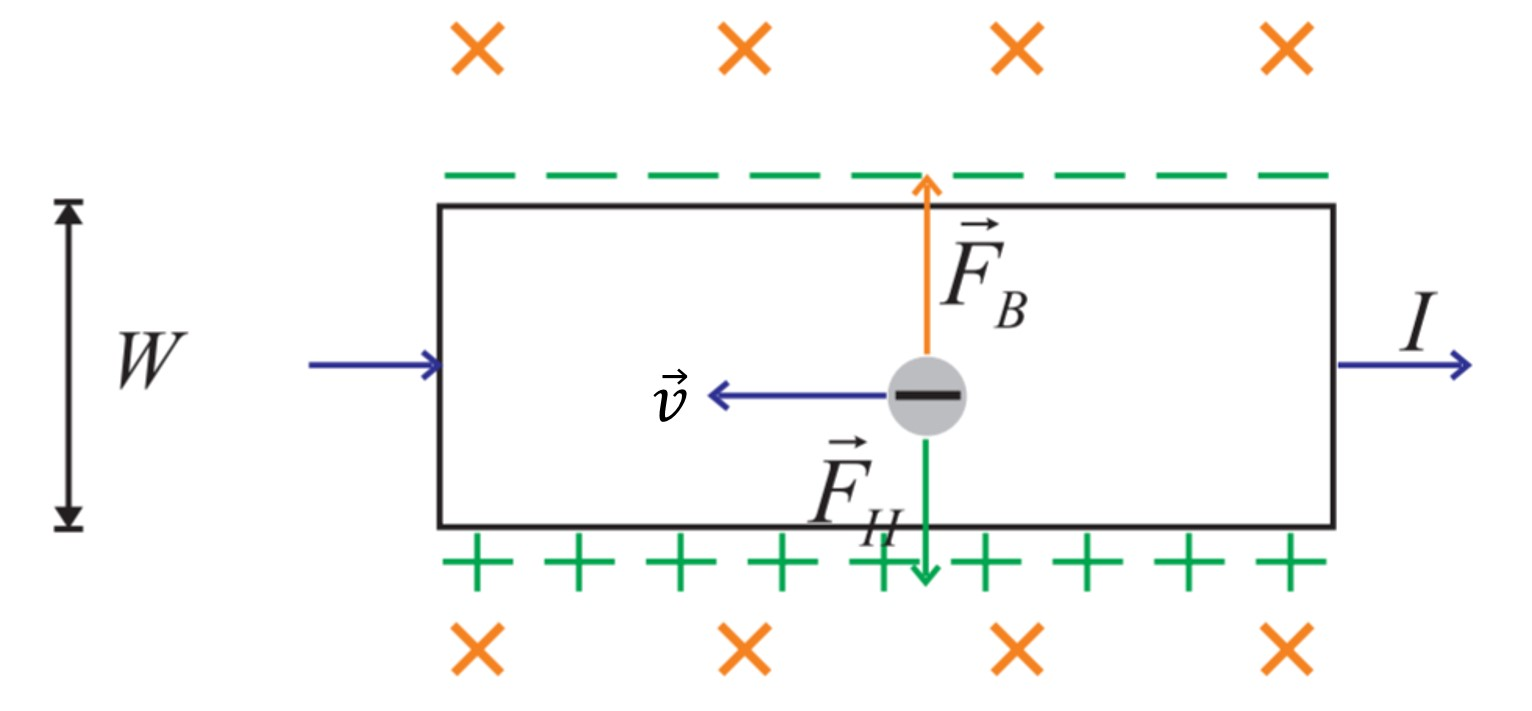
\includegraphics[scale=0.4]{notes/images/Hall-Effect.JPG}
    \caption{The Hall Effect}
\end{figure}
\FloatBarrier

The separation will stop when the magnetic force $\vec{F}_B$ experienced by the charge carriers is balanced by the force $\vec{F}_H$ caused by the electric field due to the separation of charged. We define the \textbf{Hall voltage} $\Delta V_H$ as the potential difference across the width of the wire. Therefore the electrical field strength of the electric field produced by the separated charges is \begin{equation}
    \| \vec{E} \| = \frac{\Delta V_H}{W},
\end{equation}
where $W$ is the width of the wire (or conducting strip). In equilibrium our Lorentz force is zero, hence $q(\vec{E} + \vec{v} \times \vec{B}) = \vec{0}$ meaning we can apply our special case we discussed in the previous section (see equation ??), giving us
\begin{equation}
    \frac{\Delta V_H}{W} = \| \vec{v} \| \| \vec{B}\|.
\end{equation}
Recall that current is given by $I = ne\| \vec{v} \|A$, where $n$ is the number density of the conductor. So we have
\begin{equation}
    \frac{\Delta V_H}{W} = \frac{I\| \vec{B}\|}{neA}.
\end{equation}
We note that $A = Wh$, where $h$ is the height of the conductor, giving
\begin{equation}
    \Delta V_H = \frac{I\| \vec{B}\|}{neh}.
\end{equation}

This equation has two main applications, determining the charge density of the conductor using the following equation
\begin{equation}
    n = \frac{I\| \vec{B}\|}{qh\Delta V_H}.
\end{equation}
Alternatively, we can then measure the magnetic flux density of the magnetic field provided we know the Hall voltage, current and number density of the conductor.
\begin{equation}
    \| \vec{B} \| = \frac{neh}{I} \Delta V_H.
\end{equation}

\subsection{Magnetic Force on Currents}

We've just seen that a charged particle moving through a magnetic field experiences a magnetic force $\vec{F}$. Since electric current consists of a charged particles in motion, when placed in a magnetic field, a wire will also experience a force. 

Consider a straight wire suspended in a region between two magnetic poles. The magnetic field points out of the page and is represented with dots (this is known as the ``arrow'' convention, where the dot represents an arrow head heading towards us and the arrow cross-hairs heading away from us are represented by crosses). Experimentally, we see when a downwards current passes through, the wire is deflected towards the left. However, when the current is upwards, the deflections is rightwards. (See figure \ref{fig:magnetic-field-wire-1}).

\begin{figure}[h!]
    \centering
    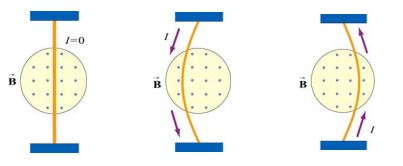
\includegraphics{notes/images/Magnetic-Field-Wire-1.JPG}
    \caption{Deflection of current-carrying wire by magnetic force}
    \label{fig:magnetic-field-wire-1}
\end{figure}
\FloatBarrier

To calculate the force exerted on the wire, consider a segment of the wire with length $\ell$ and a cross sectional area of $A$, as illustrated below. The magnetic field points into the page and is represented by crosses. 

\begin{figure}[h!]
    \centering
    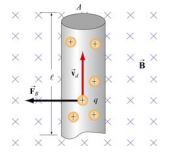
\includegraphics{notes/images/Magnetic-Field-Wire-2.JPG}
    \caption{Magnetic force on a conducting wire}
    \label{fig:magnetic-field-wire-2}
\end{figure}
\FloatBarrier

The charges moves with a mean drift velocity $\vec{v}_{drift}$. Since the total amount of charge in this segment is $Q_{total} = qnA\ell$, where $n$ is the number density of the conductor. So the total magnetic force acting on this segment is
\begin{equation}
    \vec{F} = Q_{total} (\vec{v}_{drift} \times \vec{B}) = qnA\ell (\vec{v}_{drift} \times \vec{B}) = I (\vec{\ell} \times \vec{B}).
\end{equation}
where $I = nqv_{drift}A$, and $\vec{\ell} = \ell \hat{\ell}$ is a \textit{length vector} with a magnitude $\ell$ and directed along the direction of the electric current or wire. So the magnitude of the magnetic force is given by
\begin{equation}
    \| \vec{F} \| = \| \vec{B} \| I \ell \sin \theta,
\end{equation}
where $\theta$ is the angle between the direction of current and the magnetic field lines. 

For a wire of arbitrary shape, the magnetic force can be obtained by summing over the forces acting on the small segments that make up the wire. Let the differential segment of the wire be denoted as $\mathop{\mathrm{d}\vec{s}}$. 

\begin{figure}[h!]
    \centering
    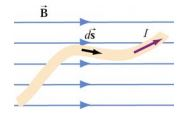
\includegraphics{notes/images/Magnetic-Field-Wire-3.JPG}
    \caption{Current-carrying wire in a magnetic field}
    \label{fig:magnetic-field-wire-3}
\end{figure}
\FloatBarrier

The magnetic force acting on the segment is 
\begin{equation}
    \mathop{\mathrm{d}\vec{F}} = I(\mathop{\mathrm{d}\vec{s} \times \vec{B}}).
\end{equation}
Thus the total force is
\begin{equation}
    \vec{F} = I \int_C \mathop{\mathrm{d}\vec{s}} \times \vec{B}.
\end{equation}
However as a magnetic field is a conservative field, the integral only depends on the initial and finial positions of the charged particle, thus we can rewrite the equation above as
\begin{equation}
    \label{eq:magnetic-force-on-wire-integral}
    \vec{F} = I \int_a^b \mathop{\mathrm{d}\vec{s}} \times \vec{B},
\end{equation}
where $a$ and $b$ represent the endpoints of the wire.

So for example, consider a curved wire carrying a current $I$ in a uniform magnetic field $\vec{B}$ as shown in figure \ref{fig:magnetic-field-wire-4}.

\begin{figure}[h!]
    \centering
    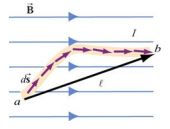
\includegraphics{notes/images/Magnetic-Field-Wire-4.JPG}
    \caption{A curved wire with a current $I$}
    \label{fig:magnetic-field-wire-4}
\end{figure}
\FloatBarrier

Using equation \ref{eq:magnetic-force-on-wire-integral}, the magnetic force on the wire is given by
\begin{equation}
    \vec{F} = I \left(\int_a^b \mathop{\mathrm{d}\vec{s}}\right) \times \vec{B} = I(\vec{\ell} \times \vec{B})
\end{equation}
where $\vec{\ell}$ is the length vector directed from $a$ to $b$. However, if the wire forms a closed loop of arbitrary shape, then the force on the loop becomes
\begin{equation}
    \vec{F} = I \int_a^a \mathop{\mathrm{d}\vec{s}} \times \vec{B}.
\end{equation}

\begin{figure}[h!]
    \centering
    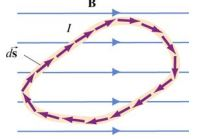
\includegraphics{notes/images/Magnetic-Field-Wire-5.JPG}
\end{figure}
\FloatBarrier

Since the set of differential length elements $\mathop{\mathrm{d}\vec{s}}$ forms a closed polygon, and their vector sum is zero. The net magnetic force on a closed loop is $\vec{F} = \vec{0}$.

\begin{experiment}
Determining magnetic flux density TODO
\end{experiment}

Alternatively, we could consider what happens when we place a rectangular loop carrying a current $I$ in the $x - y$ plane and switch on a uniform magnetic field that runes parallel to the plane of the current, that is $\vec{B} = \| \vec{B} \| \hat{i}$, as shown in the figure below.

\begin{figure}[h!]
    \centering
    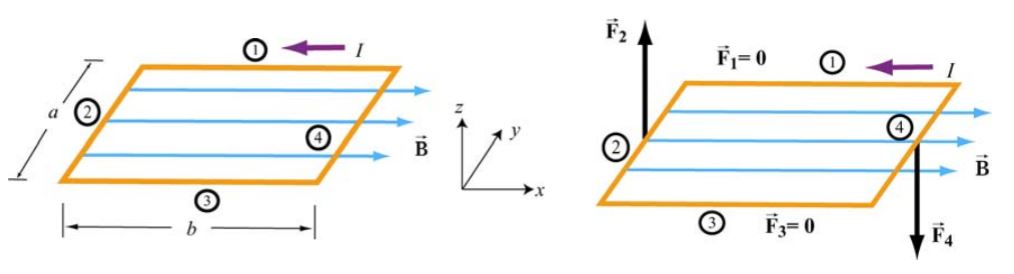
\includegraphics{notes/images/Magnetic-Feild-Current-Loop.JPG}
    \caption{(a) A rectangular current loop placed in a uniform magnetic field. (b) The magnetic forces acting on sides $2$ and $4$}
\end{figure}
\FloatBarrier

We see the magnetic forces acting on sides $1$ and $3$ vanish because their length vectors $\ell_1 = -b \hat{i}$ and $\ell_3 = b \hat{i}$ are parallel and anti-parallel to $\vec{B}$ and their cross products vanish. On the other hand, the magnetic forces acting on segments $2$ and $4$ are non-vanishing
\begin{align}
    \vec{F}_2 &= I(-a\vec{j} \times \| \vec{B} \|\hat{i}) = Ia\|\vec{B}\| \hat{k} \\
    \vec{F}_4 &= I(a\vec{j} \times \| \vec{B} \|\hat{i}) = - Ia\|\vec{B}\| \hat{k} 
\end{align}
with $\vec{F}_2$ pointing out of the page and $\vec{F}_4$ into the page. Thus, the resultant force on the rectangular loop is
\begin{equation}
    \vec{F} = \vec{F}_1 + \vec{F}_2 + \vec{F}_3 + \vec{F}_4 = \vec{0},
\end{equation}
which is a special case of equation ??, as discussed earlier. Even though the resultant force is zero, the forces $\vec{F}_2$ and $\vec{F}_4$ will produce a torque which causes the loop to rotate about the $y$-axis. 
The resultant torque (from equation ??) with respect to the center of the loop is
\begin{align}
    \vec{\tau} &= \vec{\tau}_2 + \vec{\tau}_4 \\
    &= \left(-\frac{b}{2}\hat{i} \times \vec{F}_2\right) + \left(\frac{b}{2}\hat{i} \times \vec{F}_4\right) \\
    &= Iab\|\vec{B}\|\hat{j} = IA\|\vec{B}\|\hat{j},
\end{align}
where $A=ab$ represents the area of the loop and the positive sign indicates the the rotation is clockwise about the $y$-axis. In is convenient to introduce the vector area $\vec{A} = A\hat{n}$, where $\hat{n}$ is the surface vector of the loop. The direction of $\hat{n}$ is set by the conventional right-hand rule. In this special case (i.e. when $\theta = \pi/2$) we have $\hat{n} = \hat{k}$. So the above expression for torque can be rewritten as
\begin{equation}
    \vec{\tau} = I \vec{A} \times \vec{B}. 
\end{equation}

Consider now the more general situation where the loop (or the vector area $\vec{A}$) makes an angle $\theta$ with respect to the magnetic field $\vec{B}$. 

\begin{figure}[h!]
    \centering
    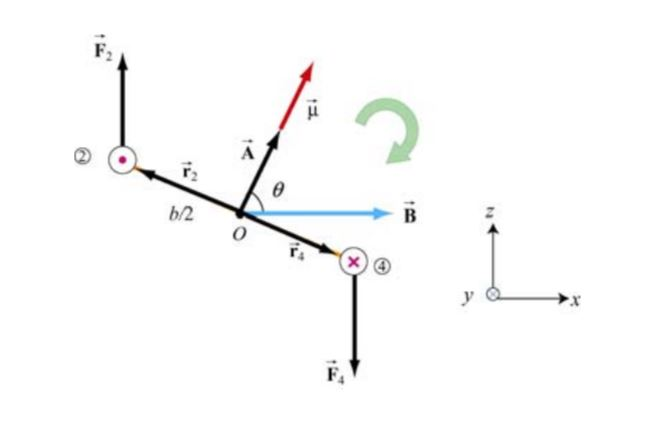
\includegraphics{notes/images/Magnetic-Fields-Current-Loop-2.JPG}
    \caption{Rotation of a rectangular current loop.}
    \label{fig:magnetic-field-current-loop-2}
\end{figure}
\FloatBarrier

From Figure \ref{fig:magnetic-field-current-loop-2}, we can see that
\begin{align}
    \vec{r}_2 &= \frac{b}{2} \left(-\cos\left(\frac{\pi}{2} - \theta\right) \hat{i} + \sin\left(\frac{\pi}{2} - \theta\right)\hat{k}\right) \\
    &= \frac{b}{2}\left(\cos(\theta) \hat{k} - \sin (\theta) \hat{i}\right) \\
    &= - \vec{r}_4
\end{align}
and the resultant torque $\vec{\tau}$ becomes
\begin{align}
    \vec{\tau} &= \vec{r}_2 \times \vec{F}_2 + \vec{r}_4 \times \vec{F}_4 \\
    &= 2 \vec{r}_2 \times \vec{F}_2 \\
    &= 2 \frac{b}{2}\left(\cos(\theta) \hat{k} - \sin (\theta) \hat{i}\right) \times \left(Ia\| \vec{B} \| \hat{k}\right) \\
    &= Iab\| \vec{B} \| \sin \theta \hat{j} \\
    &= I \vec{A} \times \vec{B}
\end{align}
For a loop consisting of $N$ turns, the resultant torque is
\begin{equation}
    \vec{\tau} = NI \vec{A} \times \vec{B}.
\end{equation}
We define the quantity $NI\vec{A}$ as the magnetic dipole moment $\vec{\mu}$:
\begin{equation}
    \vec{\mu} = NI\vec{A}
\end{equation}

\begin{figure}[h!]
    \centering
    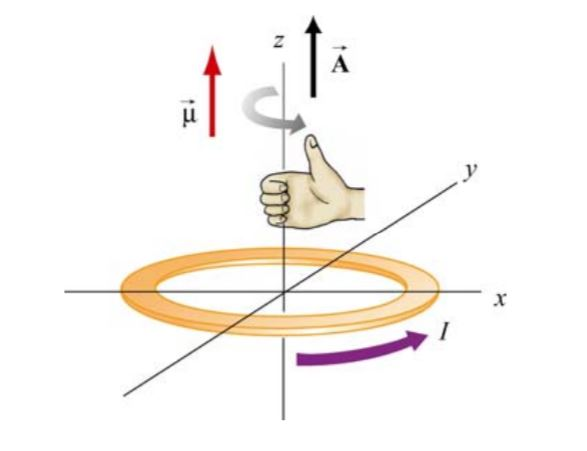
\includegraphics{notes/images/Magnetic-Fields-Current-Loop-3.JPG}
    \caption{Right-hand rule for determining the direction of $\vec{\mu}$.}
    \label{fig:magnetic-field-current-loop-3}
\end{figure}
\FloatBarrier

The direction of $\vec{\mu}$ is parallel to the vector area $\vec{A}$ (perpendicular to the plane of the loop) and is determined by a right-hand rule (figure \ref{fig:magnetic-field-current-loop-3}). Using the expression for $\vec{\mu}$, the torque exerted on the loop can be rewritten as
\begin{equation}
    \vec{\tau} = \vec{\mu} \times \vec{B}
\end{equation}

The work done by an external force to rotate the magnetic dipole from an angle $\theta_1$ to $\theta_2$ is given by (see equation ??)
\begin{align}
    W_{external} &= \int_{\theta_1}^{\theta_2} \| \vec{ \tau} \| \mathop{\mathrm{d}\theta} \\
    &= \int_{\theta_1}^{\theta_2} \| \vec{\mu} \| \vec{B} \| \sin \theta \mathop{\mathrm{d}\theta} \\
    &= \|\vec{\mu}\|\|\vec{B}\|(\cos \theta_1 - \cos \theta_2)
\end{align}
We say that $W_{external} = -W = \Delta E_p = E_{p,2} - E_{p,1} $, where $W$ is the work done by the magnetic field. Choosing $E_{p,1} = 0$ at $\theta_1 = \pi/2$, the dipole in the presence of an external field then has a potential energy of
\begin{equation}
    E_p = - \| \vec{\mu} \| \| \vec{B} \| \cos \theta = - \vec{\mu} \cdot \vec{B}.
\end{equation}

\subsubsection*{A Note on Fleming's Left-Hand Rule}

If we consider $\vec{B}$ and $\vec{v}$ being perpendicular, that is $\theta = \pi/2$ then we see that the magnetic force direction on a current-carrying wire in a uniform magnetic field is given by a left-hand rule, known as \textbf{Fleming's left-hand rule}. We use our left hands as shown in figure \ref{fig:fleming-left-hand}.

\begin{figure}[h!]
    \centering
    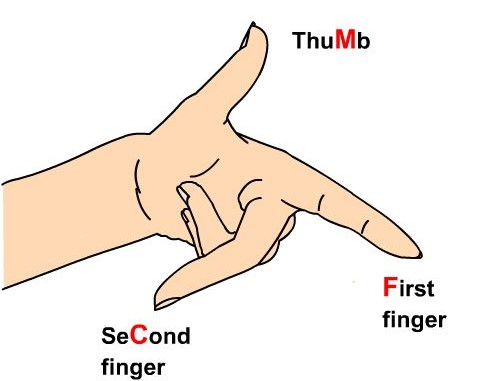
\includegraphics[scale=0.6]{notes/images/Fleming-Left-Hand.JPG}
    \caption{Fleming's left-hand rule}
    \label{fig:fleming-left-hand}
\end{figure}
\FloatBarrier

\noindent The direction of our:
\begin{itemize}
    \item \textbf{Thumb}: is the direction of our magnetic force (or motion, provided the resultant force is parallel to the magnetic force).
    \item \textbf{First finger}: is the direction of the magnetic field lines (north to south). 
    \item \textbf{Second finger}: is the direction of the \textit{convention current} through the wire. 
\end{itemize}

\section{Magnetic Fields}

\subsection{Magnetic Fields}

A moving charge can either experience a magnetic force in a magnetic field $\vec{B}$, or it can generate a magnetic field. We say the magnetic field $\vec{B}$ at point $P$ generated by a charge $q$ in space moving with a velocity $\vec{v}$ is given by
\begin{equation}
    \vec{B} = \frac{\mu_0}{4\pi} \frac{q \vec{v} \times \hat{r}}{\| \vec{r} \|^2},
\end{equation}
where $\mu_0$ is the so called \textbf{permeability of free space}. a magnetic constant, $\mu_0 = 4\pi \times 10^{-7}$ $TmA^{-1}$. This is the formal definition of a magnetic field. 

\begin{figure}[h!]
    \centering
    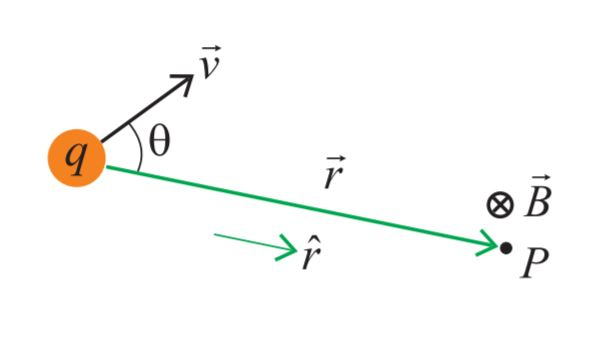
\includegraphics[scale=0.8]{notes/images/Magnetic-Field-Definition-1.JPG}
\end{figure}
\FloatBarrier

From equation ?? we can make some observations, the most obvious being that when $\theta = \pi/2$ the magnetic field experienced at point $P$ is at a maximum and when $\theta = 0, 2\pi$ the magnetic field experienced at point $P$ is at a minimum. 

\begin{figure}[h!]
    \centering
    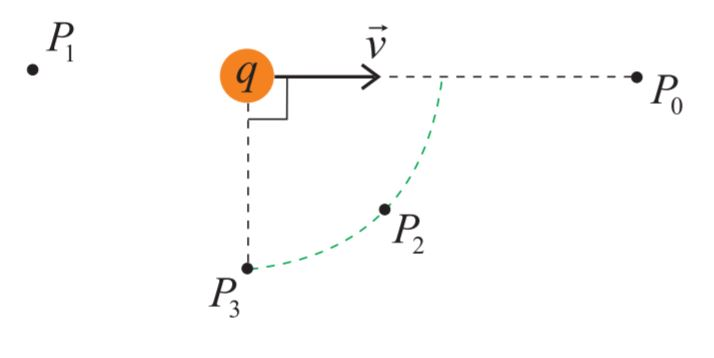
\includegraphics[scale=0.8]{notes/images/Magnetic-Field-Definition-2.JPG}
\end{figure}
\FloatBarrier

So for example, considering the figure above. The magnetic field $\vec{B}$ at $P_0$ is zero, the same can be said for the magnetic field at $P_1$. Whereas the magnetic field at $P_2$ isn't zero, however it is less than the magnetic field at $P_3$. 

Despite our definition of a magnetic field, experimentally we see that a single moving charge will \textit{not} generate a steady magnetic field. As discussed in section ??, stationary charges will generate a steady electric field $\vec{E}$, similarly, steady currents will generate a steady magnetic field $\vec{B}$. 

So a magnetic field at the point $P$ can be obtained by \textit{integrating} the contribution from individual current segments, this is known as the \textbf{principle of magnetic superposition}. By considering a small charge $\mathop{\mathrm{d}q}$ we have 
\begin{equation}
    \mathop{\mathrm{d}\vec{B}} = \frac{\mu_0}{4\pi} \frac{\mathop{\mathrm{d}q} \vec{v} \times \hat{r}}{\| \vec{r} \|^2}
\end{equation}

\begin{figure}[h!]
    \centering
    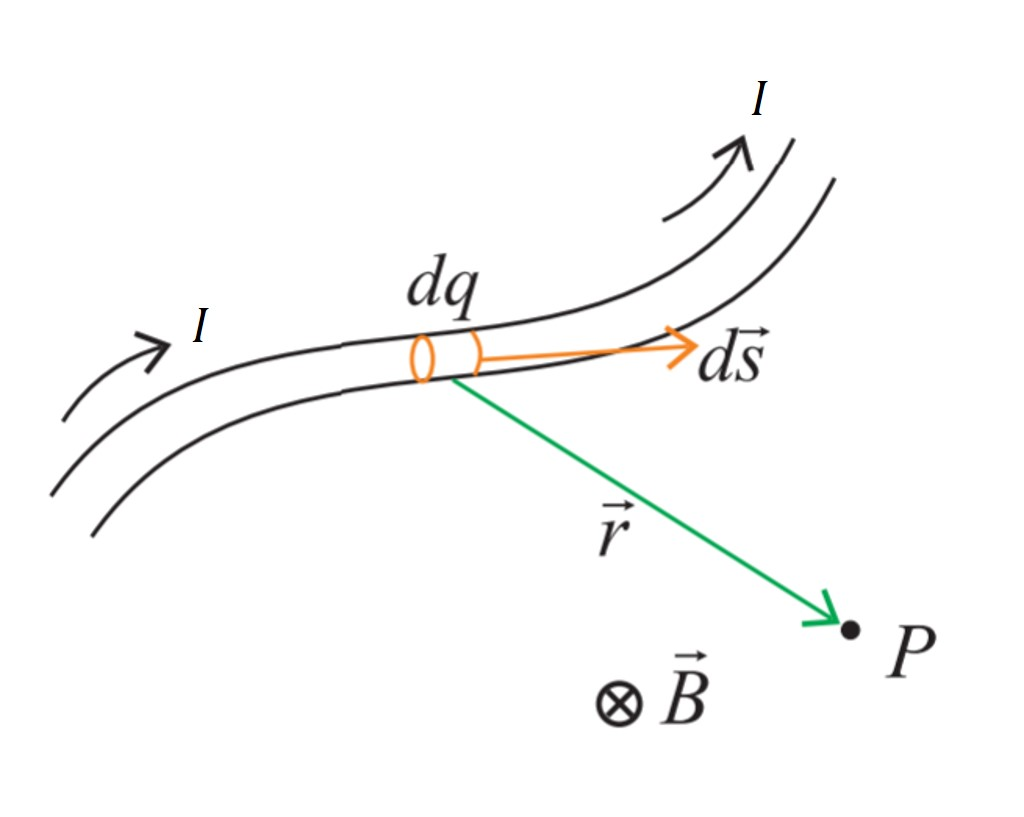
\includegraphics[scale=0.4]{notes/images/Magnetic-Superposition-1.JPG}
\end{figure}
\FloatBarrier

Notice that $\mathop{\mathrm{d}q} \vec{v} = \mathop{\mathrm{d}q} \frac{\mathop{\mathrm{d}\vec{s}}}{\mathop{\mathrm{d}t}} = I \mathop{\mathrm{d}\vec{s}}$, so 
\begin{equation}
    \mathop{\mathrm{d}\vec{B}} = \frac{\mu_0}{4\pi} \frac{I \mathop{\mathrm{d}\vec{s}} \times \hat{r}}{\| \vec{r} \|^2}.
\end{equation}
This is known as the \textbf{Biot-Savart Law} and will allow us to find the magnetic field generated by a circuit. For the current around a whole circuit
\begin{equation}
    \vec{B} = \int_C \mathop{\mathrm{d}\vec{B}} = \int_C \frac{\mu_0}{4\pi} \frac{I \mathop{\mathrm{d}\vec{s}} \times \hat{r}}{\| \vec{r} \|^2},
\end{equation}
where the curve $C$ is the topological representation of the circuit. 



We've just seen that a current in a circuit will generate a magnetic field $\vec{B}$. Consider a straight wire as shown in figure ??. We will consider an individual current segment $I \mathop{\mathrm{d}\vec{s}} = I \mathop{\mathrm{d}y} \hat{s}$ in a wire of length $\ell$ to find the magnetic field $\vec{B}$ at the point $P$. 

\begin{figure}[h!]
    \centering
    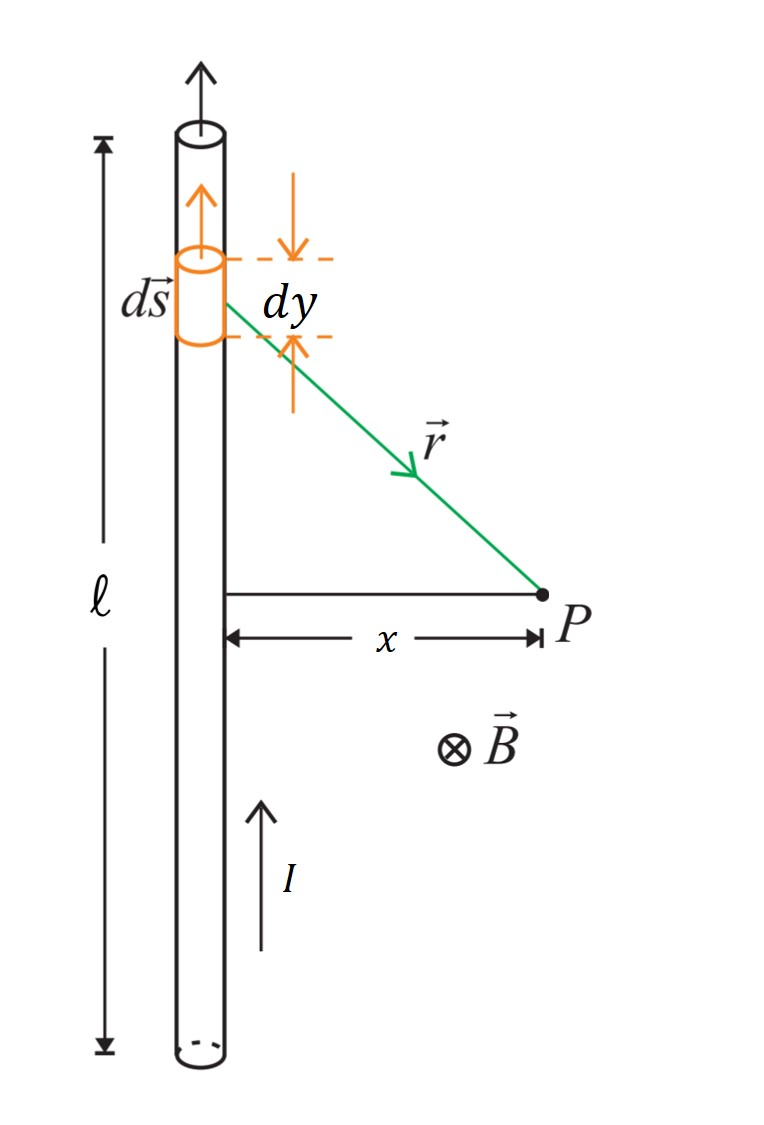
\includegraphics[scale=0.5]{notes/images/Magnetic-Field-Wire-P-1.JPG}
\end{figure}
\FloatBarrier

Abstracting the above figure geometrically gives

\begin{figure}[h!]
    \centering
    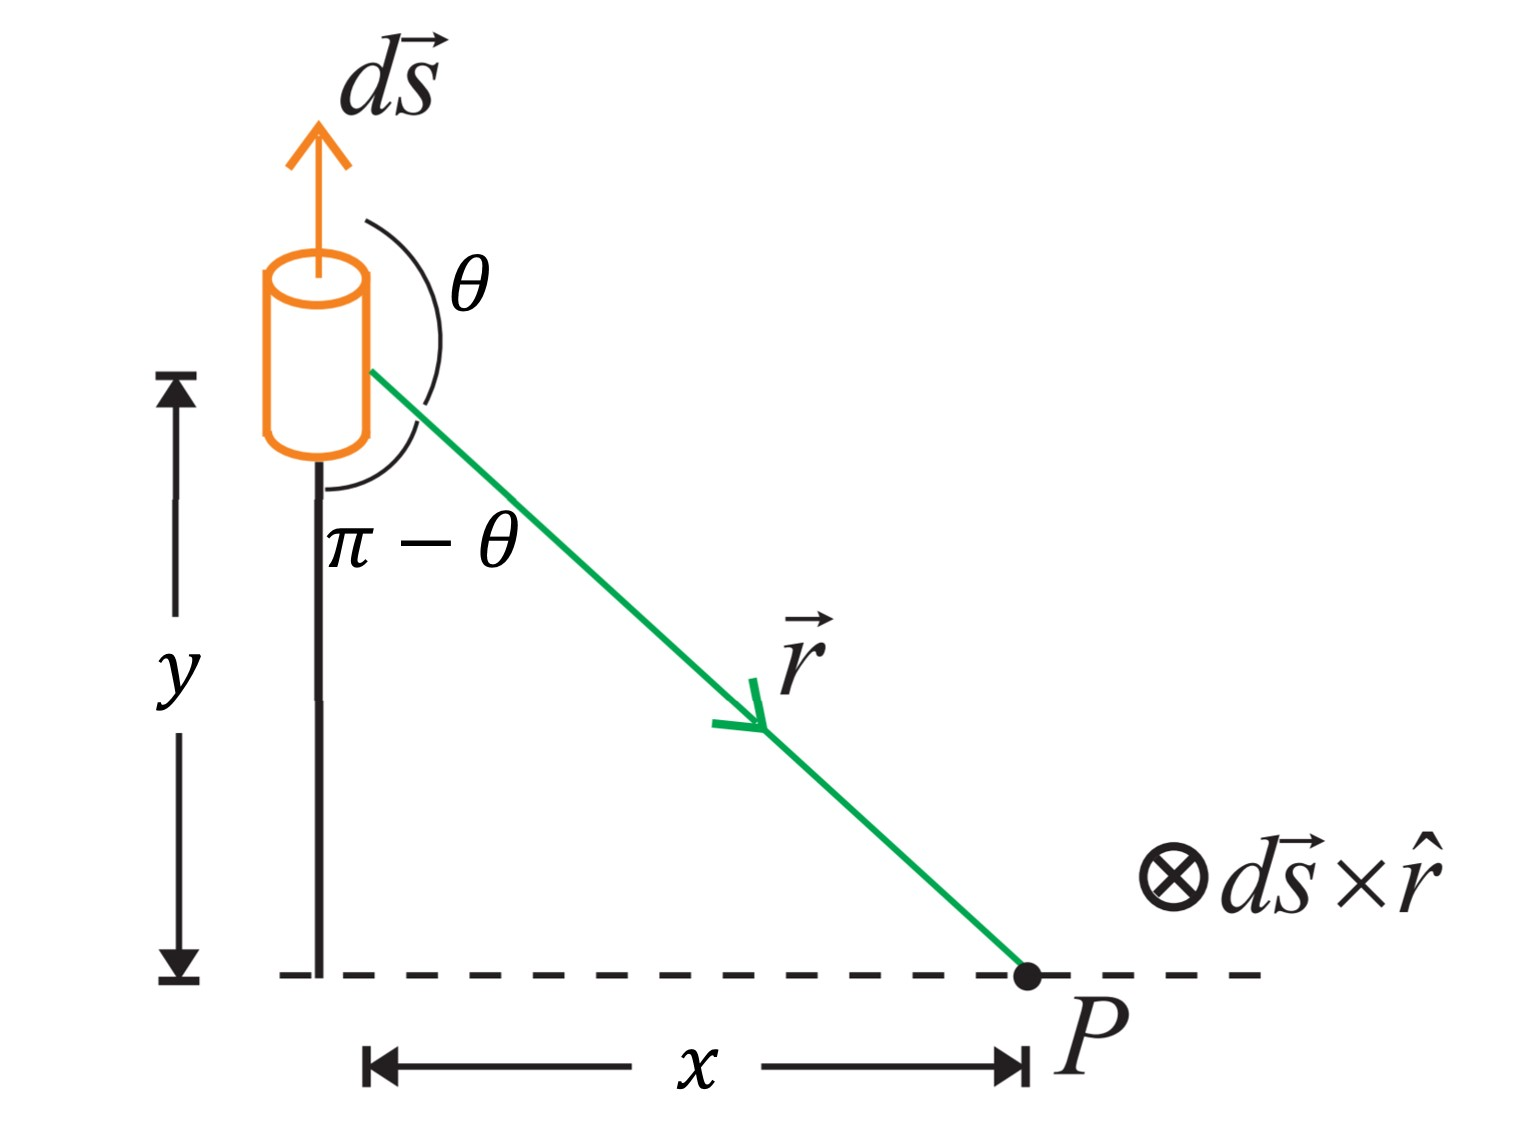
\includegraphics[scale=0.35]{notes/images/Magnetic-Field-Wire-P-2.JPG}
\end{figure}
\FloatBarrier

So the magnitude of $\mathop{\mathrm{d}\vec{s}} \times \hat{r}$ is given by
\begin{align}
    \| \mathop{\mathrm{d}\vec{s}} \times \hat{r} \| &= \mathop{\mathrm{d}y} \sin \theta \\
    &= \mathop{\mathrm{d}y} \sin (\pi - \theta) \\
    &= \mathop{\mathrm{d}y} \frac{x}{\| \vec{r} \|} \\
    &= \frac{x \mathop{\mathrm{d}y}}{\sqrt{x^2 + y^2}}
\end{align}
Applying the Biot-Savart Law produces the following relationship
\begin{align}
    \| \mathop{\mathrm{d}\vec{B}} \| &= \frac{\mu_0}{4\pi} \frac{Ix \mathop{\mathrm{d}y}}{(x^2 + y^2)^{3/2}}
\end{align}
Integrating over the current in the wire gives
\begin{equation}
    \| \vec{B} \| = \int_{-\ell/2}^{\ell/2} \frac{\mu_0}{4\pi} \frac{Ix \mathop{\mathrm{d}y}}{(x^2 + y^2)^{3/2}} = \frac{\mu_0 I x}{4 \pi} \int_{-\ell/2}^{\ell/2} \frac{\mathop{\mathrm{d}y}}{(x^2 + y^2)^{3/2}}
\end{equation}
This integral can be solved trivially via a trigonometric substitution of $y = x \tan u$, thus
\begin{equation}
    \| \vec{B} \| = \frac{\mu_0I}{4\pi x} \frac{\ell}{\sqrt{x^2 + \frac{\ell^2}{4}}}
\end{equation}
The direction of the magnetic field $\vec{B}$ can be determined via a right-hand corkscrew rule shown in the figure below. 

However, if the straight wire forms a circular current loop, then the magnetic field generated is different. In a similar fashion, let us consider a current segment $I\mathop{\mathrm{d}\vec{s}}$ on the current loop and the magnetic field generated at some point $P$, as shown in figure \ref{fig:magnetic-field-current-loop-p-1}.

\begin{figure}[h!]
    \centering
    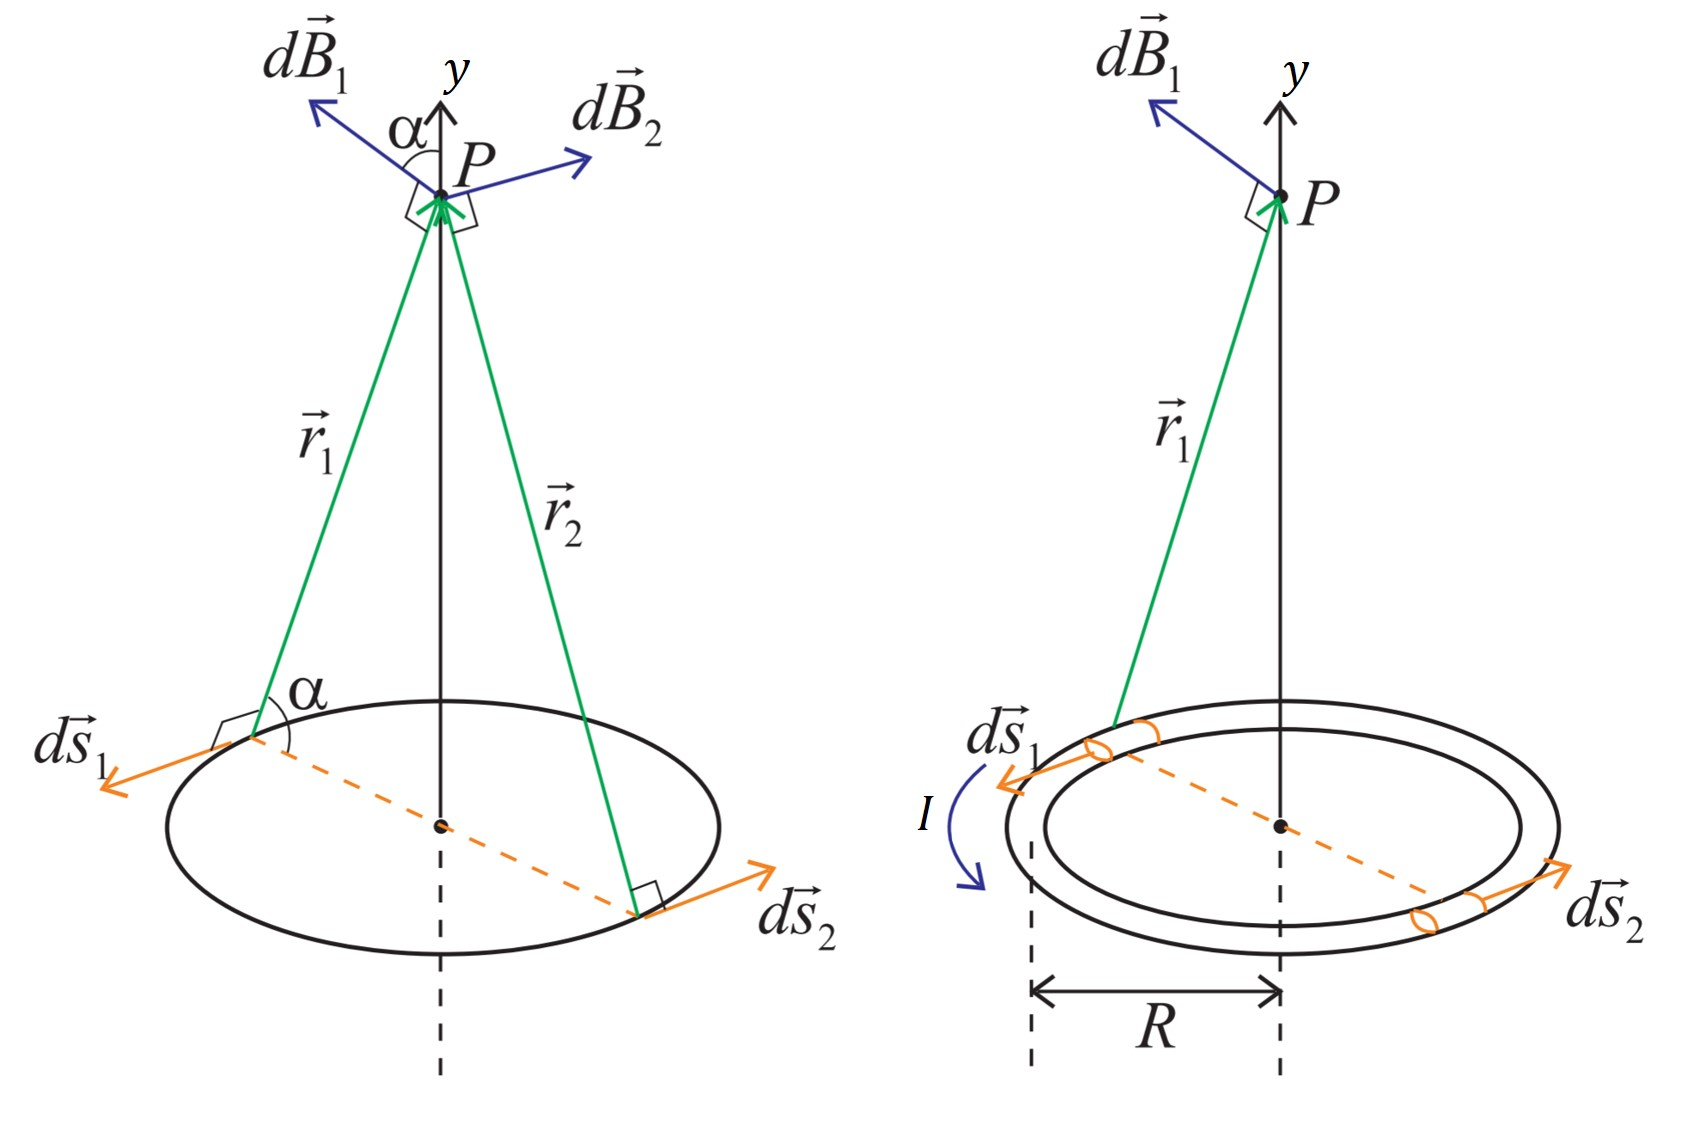
\includegraphics[scale=0.4]{notes/images/Magnetic-Feild-Current-Loop-P-1.JPG}
    \caption{(a) Geometric interpretation of two current segments in a current loop. (b) Current segment consideration in a current loop.}
    \label{fig:magnetic-field-current-loop-p-1}
\end{figure}
\FloatBarrier

Notice that for every current element $I \mathop{\mathrm{d}\vec{s}_1}$, generating a magnetic field $\mathop{\mathrm{d}\vec{B}_1}$ at point $P$, there is an opposite current element $I\mathop{\mathrm{d}\vec{s}_2}$, generating a magnetic field $\mathop{\mathrm{d}\vec{B}_2}$ such that
\begin{equation}
    \mathop{\mathrm{d}\vec{B}_1} \sin \alpha = - \mathop{\mathrm{d}\vec{B}_2} \sin \alpha
\end{equation}
Hence we only need to consider the vertical component of $\vec{B}$ needs to be considered at $P$. We also note that $\mathop{\mathrm{d}\vec{s}}$ is perpendicular to $\hat{r}$, so the magnitude of our vector product is simply $\mathop{\mathrm{d}s}$. So applying the Biot-Savart Law, gives
\begin{equation}
    \| \mathop{\mathrm{d}\vec{B}} \| = \frac{\mu_0}{4 \pi} \frac{I\mathop{\mathrm{d}s}}{\| \vec{r} \|^2}
\end{equation}
Integrating around the circuit yields our magnetic field $\vec{B}$ at $P$
\begin{align}
    \| \vec{B} \| &= \int_C \| \mathop{\mathrm{d}\vec{B}} \| \cos \alpha
\end{align}
We're multiplying the integral by $\cos \alpha$ as we're only interested in the vertical component of $\vec{B}$. Given we're considering a circular current loop, we can integrate from $0$ to $2\pi$. So 
\begin{align}
    \| \vec{B} \| &= \int_0^{2\pi} \frac{\mu_0}{4\pi} \frac{I \mathop{\mathrm{d}s}}{\| \vec{r} \|^2} \frac{R}{\| \vec{r} \|} \\
    &= \frac{IR\mu_0}{4\pi \| \vec{r} \|^3} \int_0^{2\pi} \mathop{\mathrm{d}s}
\end{align}
The integral $\int_0^{2\pi} \mathop{\mathrm{d}s}$ is simply the circumference of the circle, hence
\begin{align}
    \| \vec{B} \| &= \frac{IR^2 \mu_0}{2 \| \vec{r} \|^3} \\
    &= \frac{IR^2\mu_0}{2(R^2 + y^2)^{3/2}}
\end{align}
Similarly, the direction of the magnetic field $\vec{B}$ can be determined from the right hand corkscrew rule, where our thumb represents the direction of $\vec{B}$ and our fingers represent the direction of conventional current in the loop. Our interest in the circular current loop is because we can formally define a circular current loop as a \textbf{magnetic dipole}. We will also use this result to consider the magnetic field produce by a solenoid. 

A solenoid is commonly used to produce a \textit{strong} and \textit{uniform} magnetic field insides it's coils. Consider a solenoid of length $\ell$ consisting of $N$ turns of wire. We define $n$ as the number of turns per a unit of length, that is
\begin{equation}
    n = \frac{N}{\ell}.
\end{equation}

We note that a solenoid can be approximated by a series of tightly-packed coils of wire. This will allow us to utilise the expression for a magnetic field produced by a current loop we derived earlier.

\begin{figure}[h!]
    \centering
    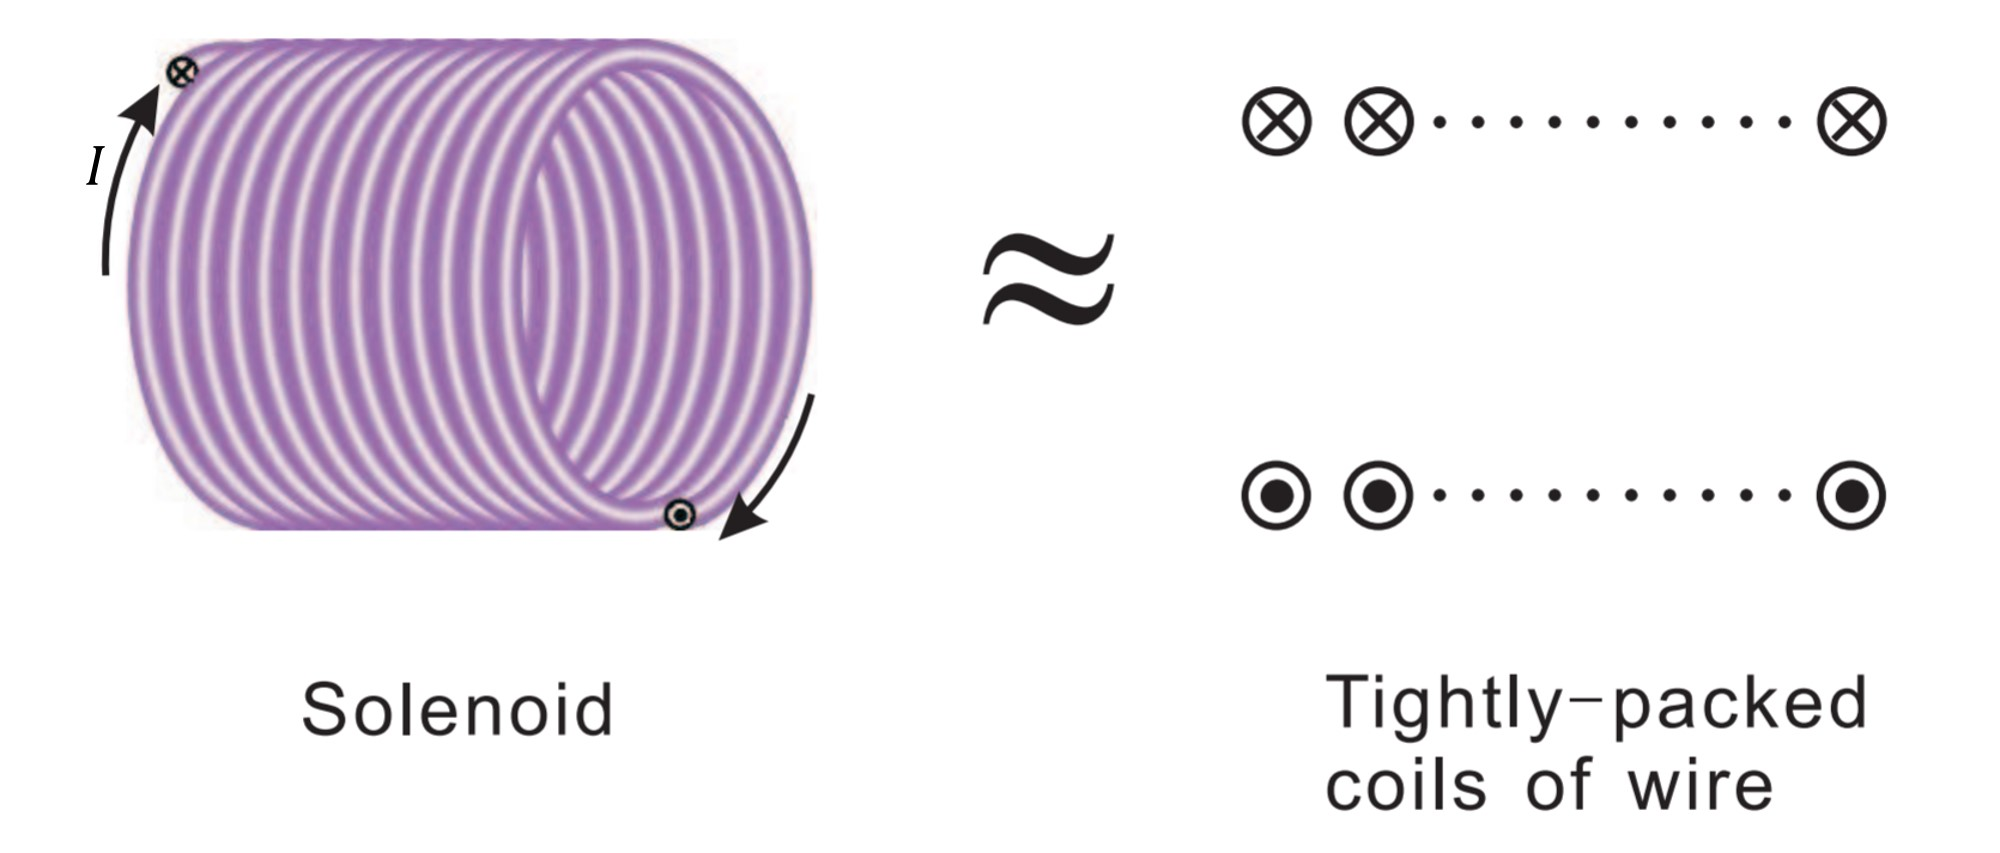
\includegraphics[scale=0.4]{notes/images/Solenoid-1.JPG}
\end{figure}

Now consider the magnetic field $\vec{B}$ at a distance $x'$ from the center of the solenoid. For a current segment we will need to consider a coil segment of length $\mathop{\mathrm{d}x}$, as shown below.

\begin{figure}[h!]
    \centering
    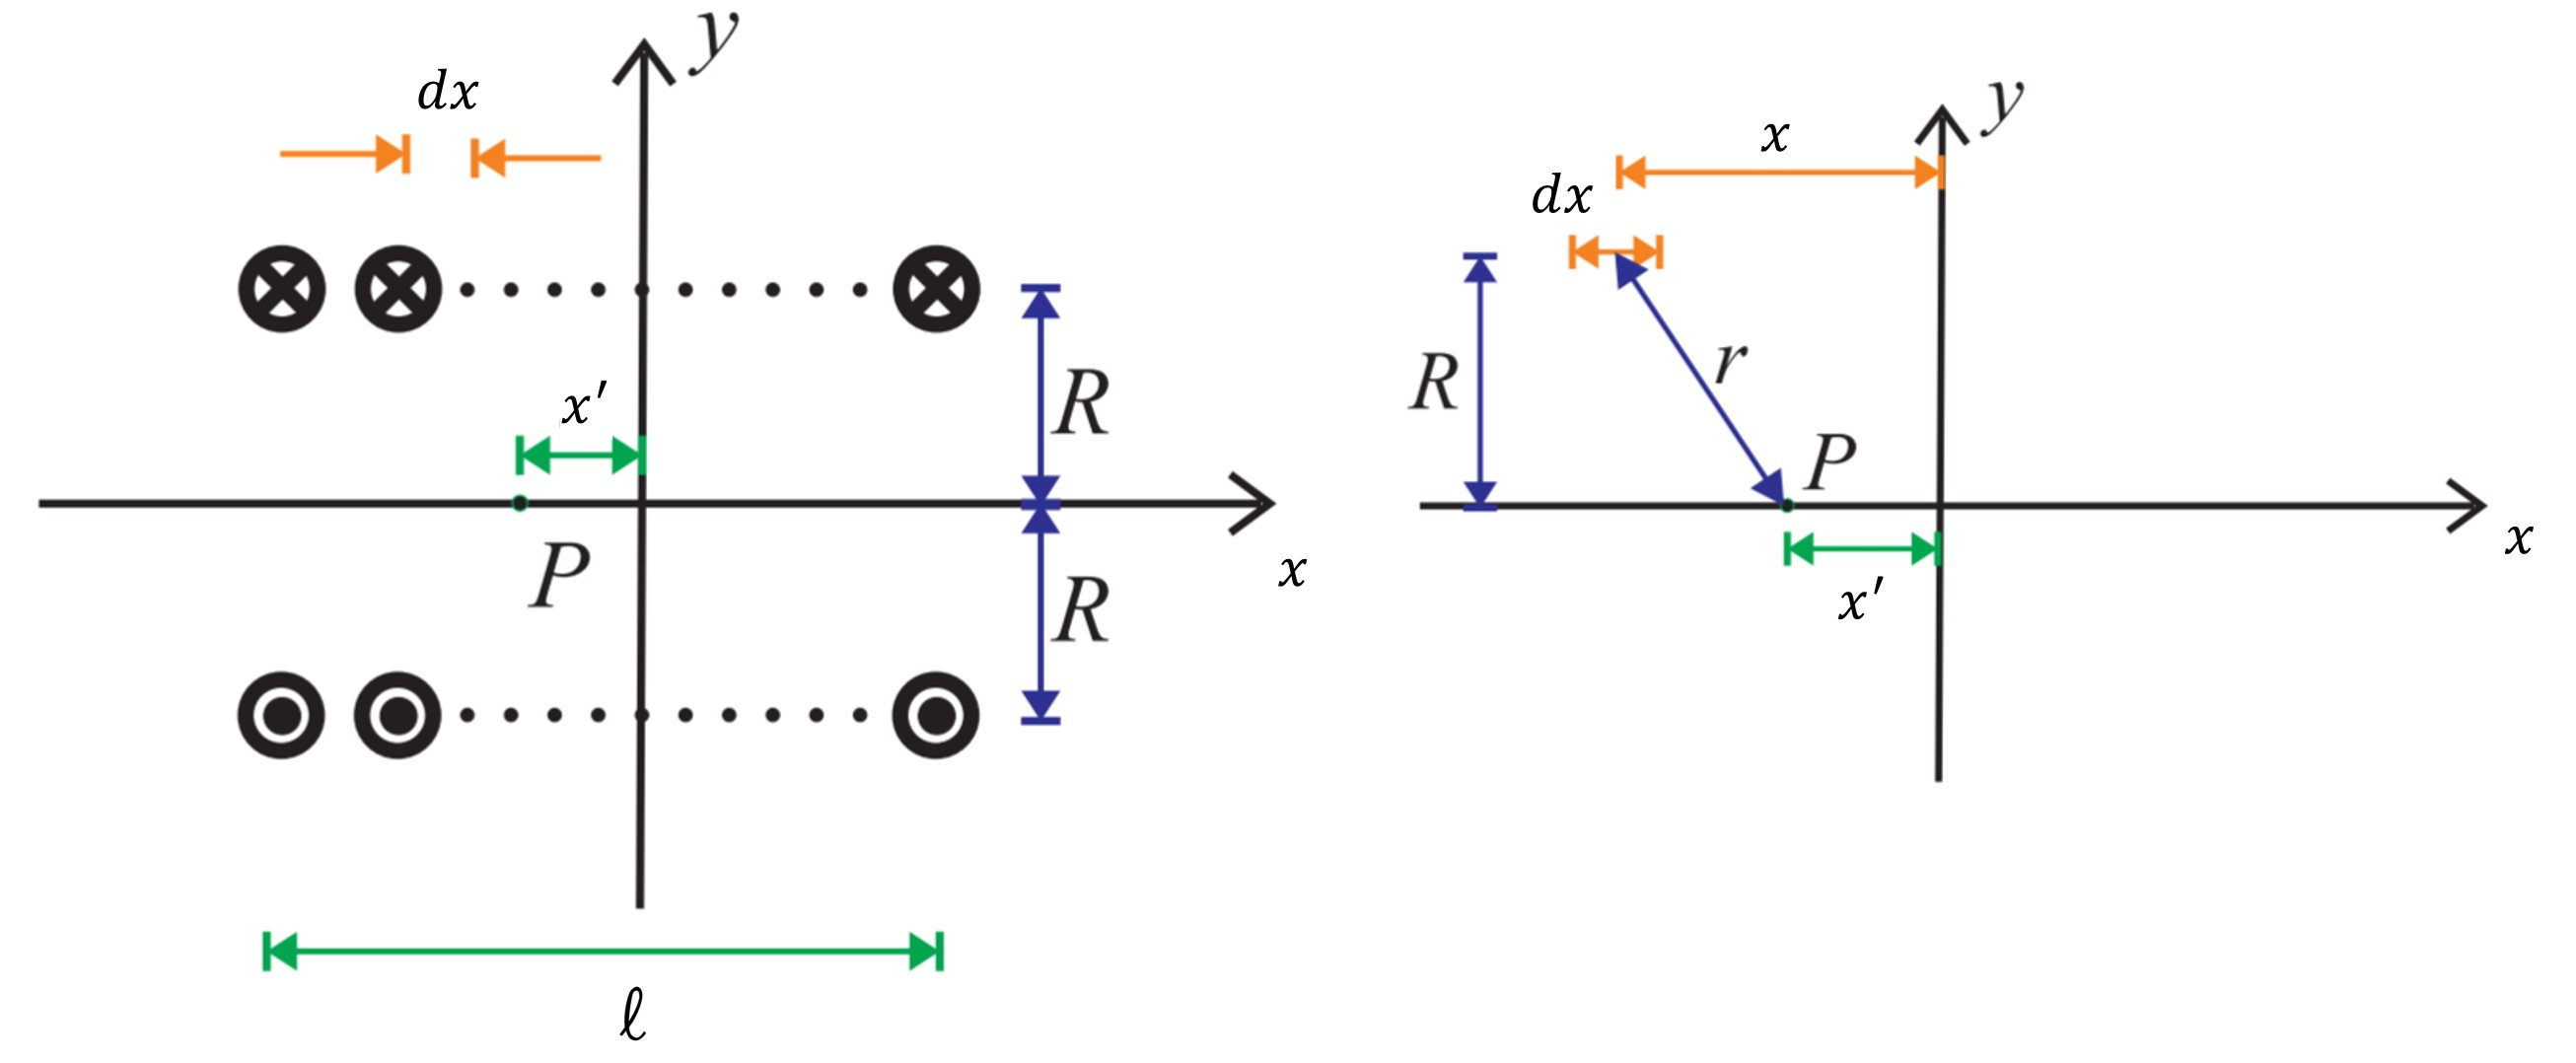
\includegraphics[scale=0.4]{notes/images/Solenoid-2.JPG}
    \caption{(a) Current segment consideration in a solenoid. (b) Geometric interpretation of current segment in a solenoid.}
\end{figure}
\FloatBarrier

Hence the number of current turns in said segment is $n \mathop{\mathrm{d}x}$. Multiplying this by the current gives us the net current $I_c$ in the coil segment, that is

\begin{equation}
    I_c = In\mathop{\mathrm{d}x}.
\end{equation}

Using the result from one coil / current loop in equation ??, we obtain the magnetic field $\vec{B}$ produced by the coil segment of length $\mathop{\mathrm{d}x}$ at a distance of $x$ from the center:
\begin{equation}
    \| \mathop{\mathrm{d}\vec{B}} \| = \frac{R^2 (In\mathop{\mathrm{d}x}) \mu_0}{2 \| \vec{r} \|^3}
\end{equation}

As clearly shown in the figure above, $\| \vec{r} \| = \sqrt{R^2 + (x - x')^2}$. So integrating over the entire solenoid gives
\begin{align}
    \| \vec{B} \| &= \int_{-\ell/2}^{\ell/2} \| \mathop{\mathrm{d}\vec{B}} \| \\
    &= \frac{IR^2n\mu_0}{2} \int_{-\ell/2}^{\ell/2} \frac{\mathop{\mathrm{d}x}}{\left(R^2 + (x - x')^2\right)^{3/2}}
\end{align}
The integral can be solved trivially via a substitution of $u = x - x'$ followed by a trigonometric substitution of $u = R\tan v$, thus
\begin{equation}
    \| \vec{B} \| = \frac{I n \mu_0}{2} \left[\frac{\frac{\ell}{2} + x'}{\sqrt{\left(\frac{\ell}{2} + x'\right)^2 + R^2}} + \frac{\frac{\ell}{2} - x'}{\sqrt{\left(\frac{\ell}{2} - x'\right)^2 + R^2}}\right]
\end{equation}
along the positive $x$ direction. The direction of the magnetic field can be determined using a right-hand corkscrew rule, as shown in the figure below. 

\begin{figure}[h!]
    \centering
    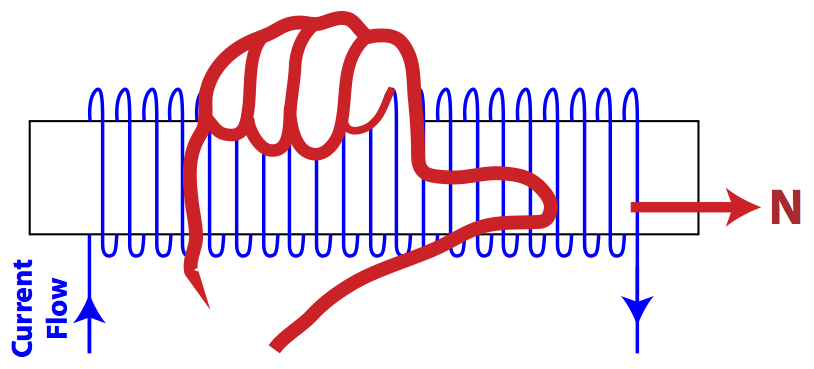
\includegraphics[scale=0.3]{notes/images/Solenoid-RHR.JPG}
    \caption{Right-hand corkscrew rule for a solenoid.}
\end{figure}
\FloatBarrier

\subsection{Ampere's Law}

In our study of magnetism we often try to calculate the magnetic field $\vec{B}$ for highly symmetrical objects, such as a wire, circular current loop or solenoid. So far we've been considering each object independently and applying the Biot-Savart Law. However, we can apply \textbf{Ampere's Law} instead which states the line integral around a closed curve $C$, referred to as an \textbf{Amperian curve}, of a magnetic field $\vec{B}$ with respect to displacement $\vec{s}$ is $I_c \mu_0$, that is
\begin{equation}
    \int_C \vec{B} \cdot \mathop{\mathrm{d}\vec{s}} = I_c \mu_0,
\end{equation}
where $I_c$ is the net current that penetrates the area bounded by the curve $C$. 
\subsubsection*{A note on convention} 
We commonly use the right-hand corkscrew rule to determine the \textit{sign} of the current. So for example, consider the currents $I_1, I_2, I_3$ and $I_4$ and the Amperian curve $C$ as shown in figure \ref{fig:ampere-law-1}. We have
\begin{align}
    \int_C \vec{B} \cdot \mathop{\mathrm{d}\vec{s}} &= \mu_0 (I_1 - I_3 + I_4 - I_4) \\
    &= \mu_0 (I_1 - I_3)
\end{align}

\begin{figure}[h!]
    \centering
    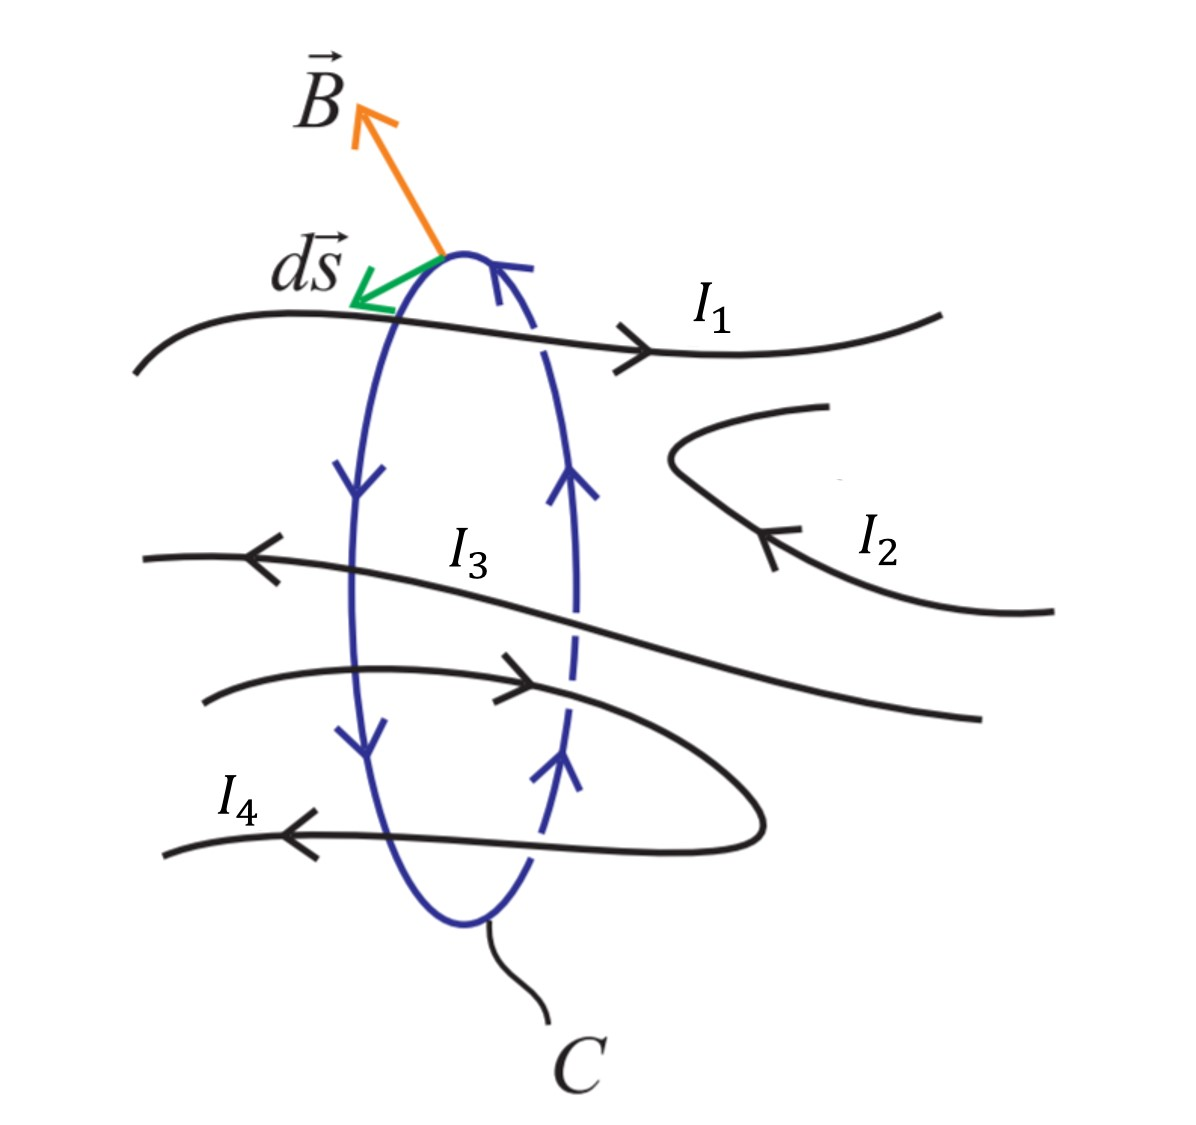
\includegraphics[scale=0.4]{notes/images/Ampere-Law-1.JPG}
    \caption{Ampere's Law Example}
    \label{fig:ampere-law-1}
\end{figure}
\FloatBarrier

We will now consider our previous results for the magnetic field of a wire and solenoid, however, we will consider them with respect to Ampere's law instead of the Biot-Savart law. 

For a straight wire, construct an Amperian curve $C$ of radius $x$ as illustrated below.

\begin{figure}[h!]
    \centering
    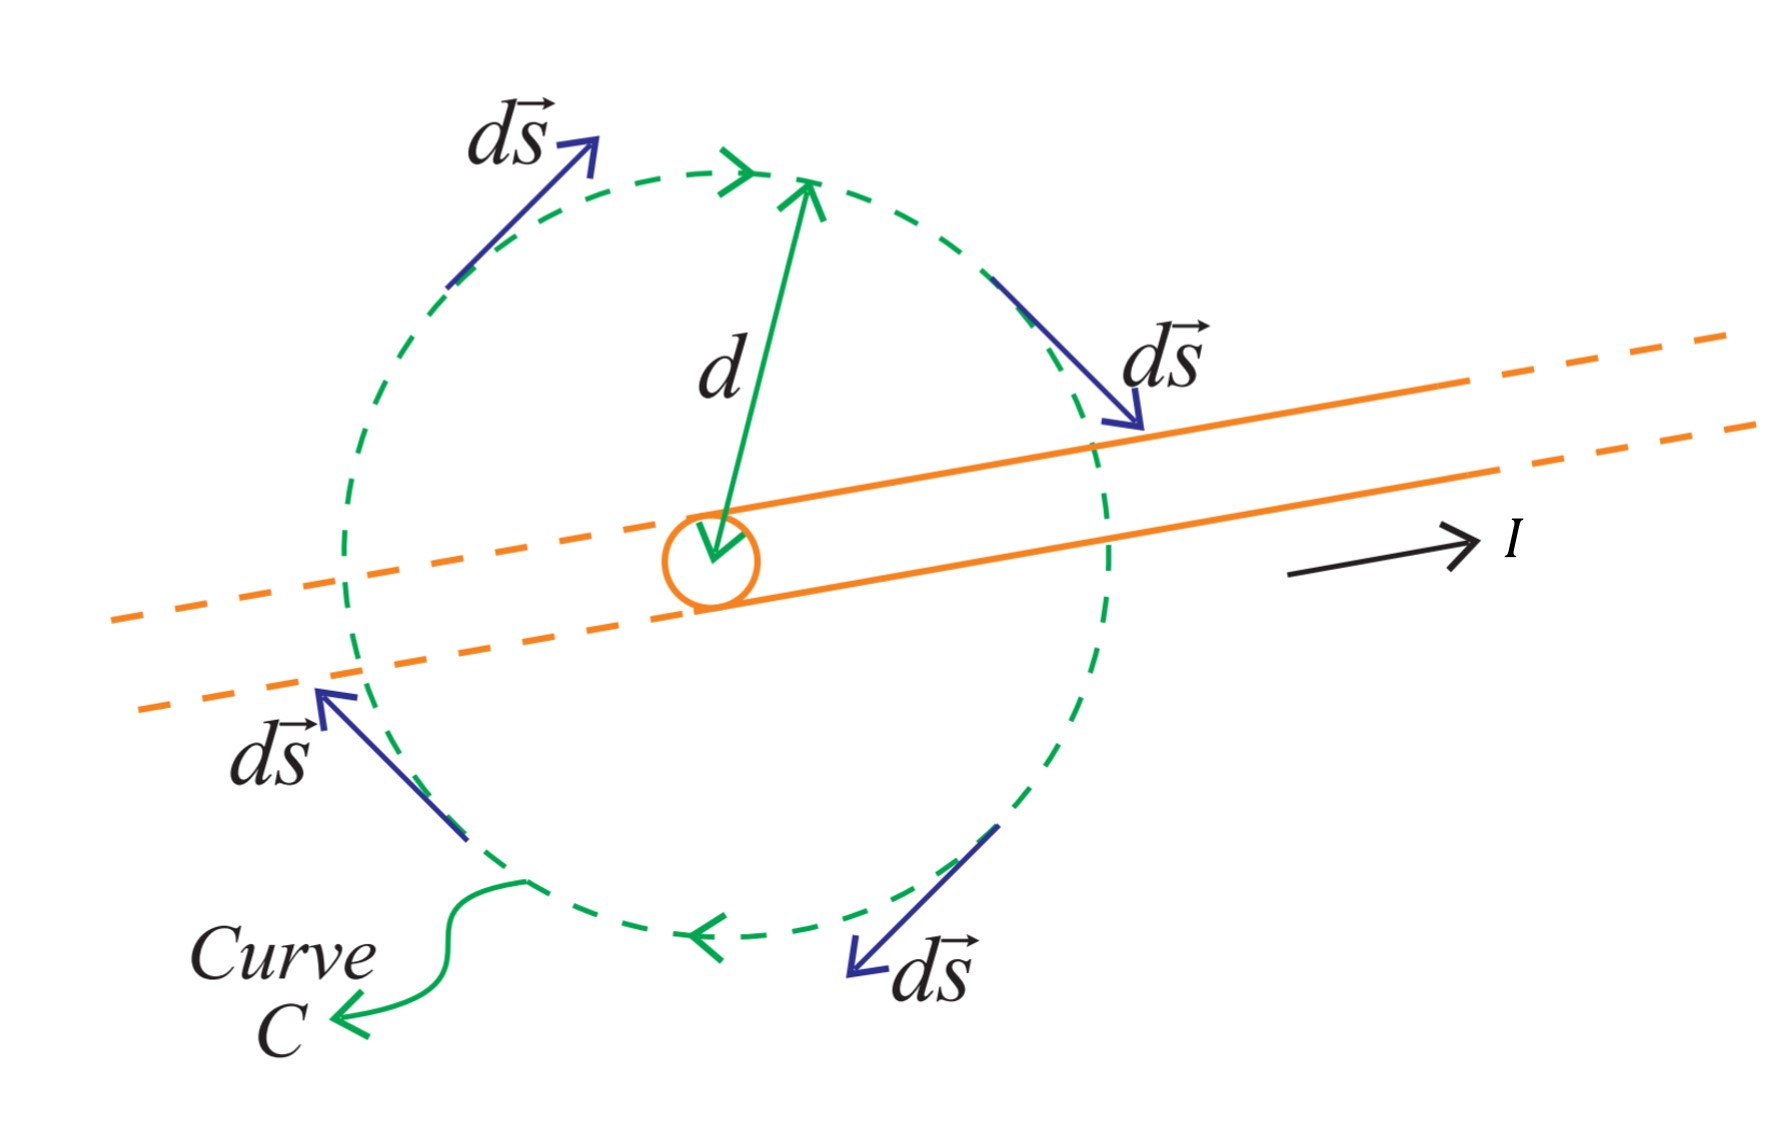
\includegraphics[scale=0.3]{notes/images/Ampere-Law-Straight-Wire.JPG}
\end{figure}
\FloatBarrier

By a symmetry argument (and our previous results) we know the magnetic field $\vec{B}$ only has tangential components to our curve $C$. Let us take $\mathop{\mathrm{d}\vec{s}}$ to be the tangential component of the curve $C$, therefore
\begin{equation}
    \vec{B} \cdot \mathop{\mathrm{d}\vec{s}} = \| \vec{B} \| \mathop{\mathrm{d}s},
\end{equation}
hence
\begin{align}
    \int_C \vec{B} \cdot \mathop{\mathrm{d}\vec{s}} &= \| \vec{B} \| \int_C \mathop{\mathrm{d}s} \\
    &= \| \vec{B} \| \cdot 2\pi x
\end{align}
So it follows from Ampere's law that
\begin{equation}
    \| \vec{B} \| = \frac{\mu_0 I}{2 \pi x}.
\end{equation}
However this differs from equation ??. Why? In our symmetry argument we only considered the \textbf{ideal case}, that is the length of the wire $\ell$ is really greater than $x$, that is $\ell \gg x$. Applying the same assumption to equation ?? will produce equation ??, thus validating our results. 

\begin{figure}[h!]
    \centering
    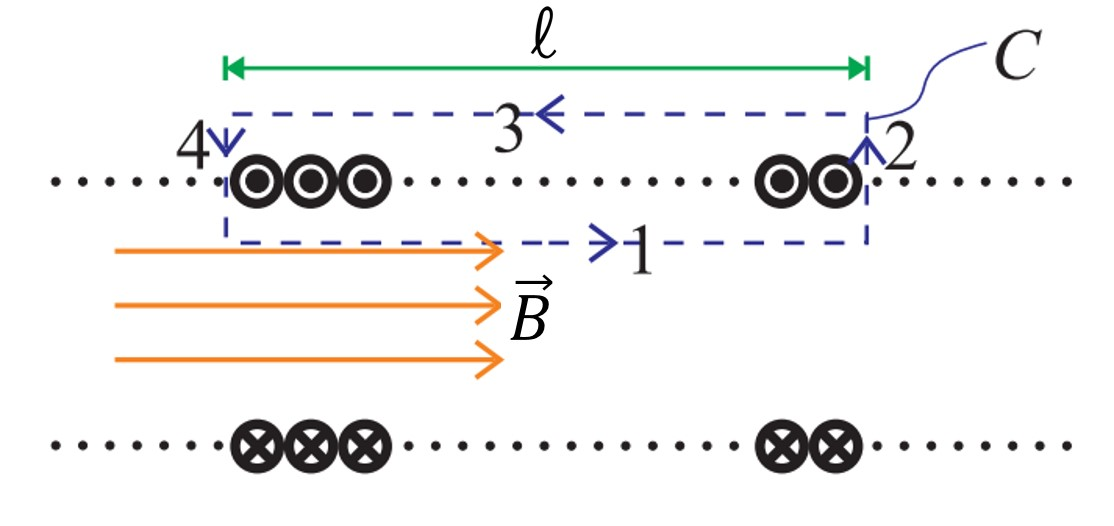
\includegraphics[scale=0.5]{notes/images/Amperes-Law-Solenoid.JPG}
    \caption{Ampere's Law applied to an ideal solenoid.}
    \label{fig:amperes-law-solenoid}
\end{figure}
\FloatBarrier

In a similar fashion, consider the Amperian curve $C$ constructed around a solenoid, as shown in figure \ref{fig:amperes-law-solenoid}. Let us dissect our curve into four segments $1,2,3$ and $4$. Using the linearity of the integral, we can write our line integral as
\begin{equation}
    \int_C \vec{B} \cdot \mathop{\mathrm{d}\vec{s}} = \int_1 \vec{B} \cdot \mathop{\mathrm{d}\vec{s}} + \int_2 \vec{B} \cdot \mathop{\mathrm{d}\vec{s}} + \int_3 \vec{B} \cdot \mathop{\mathrm{d}\vec{s}} + \int_4 \vec{B} \cdot \mathop{\mathrm{d}\vec{s}}
\end{equation}
Given we're considering an ideal solenoid, the uniform magnetic field only exists inside the solenoid, thus
\begin{equation}
    \int_3 \vec{B} \cdot \mathop{\mathrm{d}\vec{s}} = 0.
\end{equation}
Similarly, we can say
\begin{equation}
    \int_2 \vec{B} \cdot \mathop{\mathrm{d}\vec{s}} = - \int_4 \vec{B} \cdot \mathop{\mathrm{d}\vec{s}}
\end{equation}
So
\begin{equation}
    \int_C \vec{B} \cdot \mathop{\mathrm{d}\vec{s}} = \int_1 \vec{B} \cdot \mathop{\mathrm{d}\vec{s}} = \| \vec{B} \| \ell = \mu_0 I_c
\end{equation}
But $I_c = NI = n\ell I$, therefore the magnetic flux density for an ideal solenoid is given by
\begin{equation}
    \| \vec{B} \| = \mu_0 n I
\end{equation}

\subsection{Faraday's Law of Induction}

In the previous chapter, we have shown how a steady electric current can give rise to a stead magnetic field (due to the link between magnetic fields and electric field). However, we could also ask whether a steady magnetic field can give a steady electric current? Or whether a changing magnetic field can give a steady electric current. We will shortly see that the latter is correct, but first we must define magnetic flux.

\begin{definition}{(\textbf{Magnetic Flux})}
\textit{The magnetic flux $\phi$ through the surface $S$ is defined as}
\begin{equation}
    \phi = \int_S \vec{B} \cdot \mathop{\mathrm{d}\vec{A}},
\end{equation}
\textit{measured in Weber ($Wb$).}
\begin{figure}[h!]
    \centering
    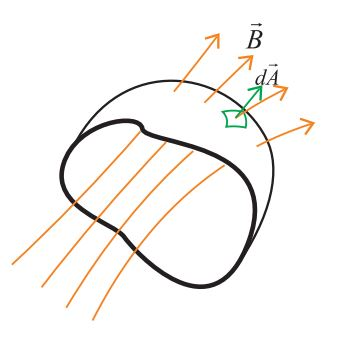
\includegraphics[scale=0.5]{notes/images/Magnetic-Flux.JPG}
\end{figure}
\FloatBarrier
\textit{The graphical, and perhaps more intuitive, definition of magnetic flux is the number of magnetic field lines passing through the surface $S$, as shown in the figure above.}
\end{definition}

To explain induction, let us consider a simple bar magnet with a magnetic field $\vec{B}$. We move a straight wire near the magnetic, as the magnetic flux $\phi$ through the wire changes (due to the movement of the wire) an emf is induced in the conductor. This effect is amplified if we use a coil of wire. For a coil of $N$ turns, the emf induced is $N$ times greater than for single turn of wire.

\begin{theorem}{(\textbf{Faraday's Law of Induction})}
\textit{The magnitude of the induced emf $\varepsilon$ is directly proportional to the rate of change of magnetic flux $\phi$ and the number of turns $N$ in the conductor.}
\begin{equation}
    | \varepsilon | = N \left|\frac{\mathop{\mathrm{d}\phi}}{\mathop{\mathrm{d}t}}\right|
\end{equation}
\begin{proof}
\textit{From Faraday's Law, we have}
\begin{equation*}
    | \varepsilon | \propto N \left|\frac{\mathop{\mathrm{d}\phi}}{\mathop{\mathrm{d}t}}\right|.
\end{equation*}
\textit{The relationship above can be written with a constant of proportionality $k$.}
\begin{equation*}
    | \varepsilon | = kN \left|\frac{\mathop{\mathrm{d}\phi}}{\mathop{\mathrm{d}t}}\right|
\end{equation*}
\textit{We can say $k = 1$, by definition the unit of emf, the volt, as the emf induced by a single wire moving through a single field line of the magnetic field $\vec{B}$ per a second. Allowing Faraday's Law of Induction to be written mathematically as}
\begin{equation*}
    | \varepsilon | = N \left|\frac{\mathop{\mathrm{d}\phi}}{\mathop{\mathrm{d}t}}\right|
\end{equation*}
\end{proof}
\end{theorem}

We must also note that the induced emf drives a current throughout the circuit, similar to the function of a cell. However, the difference here is that the induced emf is distributed throughout the circuit. The consequence is that we \textbf{cannot} define a potential difference between any two points in the circuit (\textit{A2 Physics = Wrong Physics. Slow clap.}). We can justify this by considering a circular current loop, as shown below.

If we consider the potential difference from $A$, going to $B$, we get $V_A > V_B$. However, if we consider the potential difference from $B$, going to $A$ then we get $V_B > V_A$. Thus we cannot define $\Delta V_{AB}$!

\subsection{Lenz' Law}

\begin{theorem}{(\textbf{Lenz' Law})}
\textit{Lenz' law states that the flux of the magnetic field due to the induced current \textbf{opposes} the change in flux that causes the induced current. Mathematically, Lenz' law can be combined with Faraday's law of induction to give}
\begin{equation}
    \varepsilon = -N\frac{\mathop{\mathrm{d}\phi}}{\mathop{\mathrm{d}t}}
\end{equation}
\end{theorem}

As an example of Lenz' law, let us consider a circuit with an induced emf and the resulting induced current in the anticlockwise direction with $\vec{B}$ directed out from the page and the area of the circuit is decrease. Hence the flux through the circuit is decreasing in the outwards direction. The induced current $I$ produced it's own magnetic field $\vec{B}_I$ whose direction may be determined by the right-hand grip rule. The result is that the magnetic field due to the induced current is also directed outwards within the circuit. 

If the rate of change of magnetic flux is greater than zero, then the magnetic flux $\phi$ increase. From Faraday's law of induction we know that an emf $\varepsilon$ is induced with a resulting induced current. A magnetic field $\vec{B}_I$ from the induced current is produced, causing a change in $\phi$ such that $\phi$ decreases, thus restoring equilibrium (\textit{one could say a regression to the mean. \textbf{Insert teen wolf meme here}}). It is as though nature, through this induced field $\vec{B}_I$ tried to compensate for the reduction in flux due to the applied field $\vec{B}$. 

We can also say that Lenz' law is a consequence from the principle of conservation of energy, consider the following: A bar magnetic with a magnetic field $\vec{B}$ (directed in direction of motion) moves towards a loop of wire. This gives rise to a change in flux through the wire. There are two possible outcomes, the current has an anticlockwise direction or a clockwise direction (by the pigeonhole principle). If the current is clockwise, then the magnet is accelerated due to the rule of action and energy is not conserved. However, if the current is clockwise in direction, then the magnet is decelerated due to the rule of action and energy is conserved. 

\begin{figure}[h!]
    \centering
    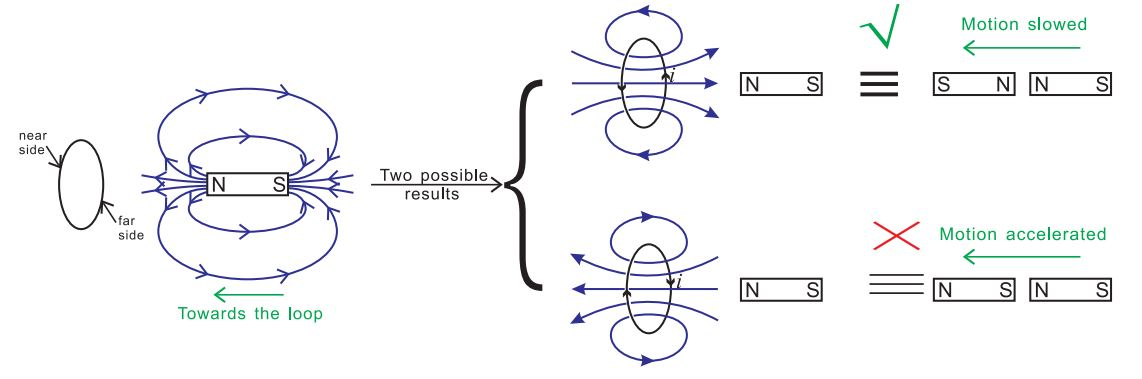
\includegraphics[scale=0.5]{notes/images/Lenz-1.JPG}
    \caption{Lenz' Law and the Conservation of Energy}
\end{figure}
\FloatBarrier

\subsubsection*{Generators}

Let us consider a generator, a circuit loop that is rotating at a constant angular velocity $\omega$ and a magnetic field $\vec{B}$ pointing into the plane of the diagram. The source of rotation is type a steam powered turbine, however water falling from a dam is an example of a different source. 

\begin{figure}[h!]
    \centering
    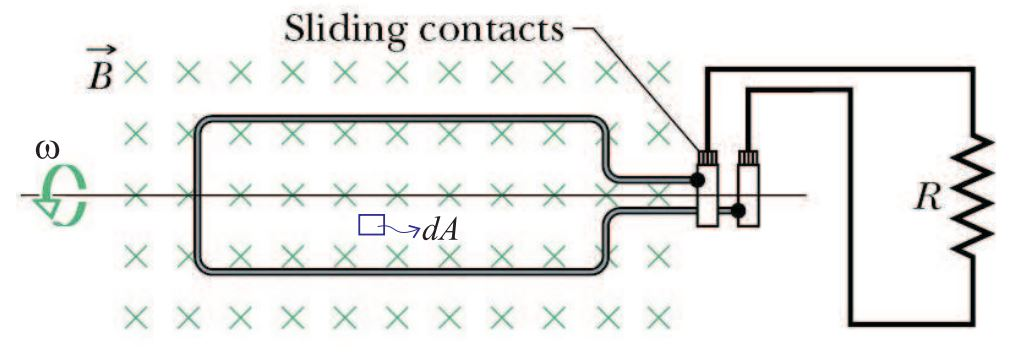
\includegraphics[scale=0.5]{notes/images/Generator-1.JPG}
\end{figure}
\FloatBarrier

Consider a small area $\mathop{\mathrm{d}\vec{A}}$ on the surface $S$ of the circuit loop and the magnetic field $\vec{B}$.

\begin{figure}[h!]
    \centering
    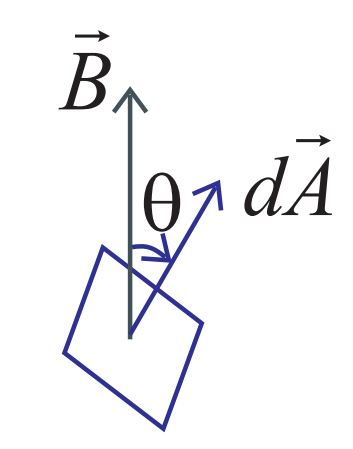
\includegraphics[scale=0.3]{notes/images/Generator-2.JPG}
\end{figure}
\FloatBarrier

From the definition of magnetic flux, we have
\begin{align}
    \phi &= \int_S \vec{B} \cdot \mathop{\mathrm{d}\vec{A}} \\
    &= \|\vec{B} \|A \cos \theta
\end{align}
where $\phi$ is the flux through a single turn of the coil and $A$ is the area of the loop. So by Faraday's law of induction, the induced emf is given by
\begin{equation}
    \varepsilon = -N \frac{\mathrm{d}}{\mathop{\mathrm{d}t}} \left(\|\vec{B} \|A \cos \theta\right)
\end{equation}
Notice that $\theta$ is a time dependent variable and recall that $\theta = \omega t$, so 
\begin{equation}
    \varepsilon = N \|\vec{B}\| A \omega \sin \omega t
\end{equation}


\subsection{Transformers}